%--------------------------------------------------------------------------------
%	PAQUETES
%--------------------------------------------------------------------------------
\documentclass[twoside]{report}
\usepackage{listings}
\renewcommand{\lstlistingname}{Código}
\renewcommand\lstlistlistingname{Índice de códigos}
\usepackage[usenames,dvipsnames]{color}

\usepackage{graphicx}
\usepackage{subfig}
\usepackage[spanish, es-tabla]{babel}
\usepackage[hidelinks]{hyperref}
\usepackage{pdfpages}
\usepackage{amsmath}
\usepackage{booktabs}
\usepackage{setspace}
\usepackage{relsize}
\usepackage[justification=centering]{caption}
\usepackage{float}
\usepackage{multirow}
\usepackage[table,xcdraw]{xcolor}

\lstset{texcl=true}
\counterwithout{footnote}{chapter} %Números pie de página

\usepackage{fancyvrb}

%--------------------------------------------------------------------------------
%	ESTILO DEL DOCUMENTO
%--------------------------------------------------------------------------------
% SANGRÍA
\parindent 0pt

% MÁRGENES
\usepackage[margin=1.5in, top=1in]{geometry}

% CABECERA Y PIE
\usepackage{fancyhdr}

\fancyhead{}
\fancyfoot{}
\fancyhead[LE,RO]{\thepage}
\fancyhead[LO]{\slshape \rightmark}
\fancyhead[RE]{\slshape \leftmark}
\pagestyle{fancy}

% FORMATO CÓDIGO R
\definecolor{mygray}{gray}{0.95}
\lstset{
	language=R,
	basicstyle=\small\ttfamily,
	%numbers=left,
	%numberstyle=\scriptsize\color{Blue},
	%stepnumber=1,
	%numbersep=5pt,
	backgroundcolor=\color{mygray},
	showspaces=false,
	showstringspaces=false,
	showtabs=false,
	%frame=single,
	rulecolor=\color{black},
	tabsize=2,
	captionpos=b,
	breaklines=true,
	breakatwhitespace=false,
	keywordstyle=\color{RoyalBlue},
	commentstyle=\color{YellowGreen},
	stringstyle=\color{ForestGreen}
}

% BIBLIOGRAFIA
\usepackage[backend = biber, style = apa, autocite = inline,%
            defernumbers = true]{biblatex}
\addbibresource{references.bib}


\begin{document}
	
%--------------------------------------------------------------------------------
%	PORTADA
%--------------------------------------------------------------------------------
\includepdf{portada.pdf} % Portada 1(obligatoria)

\shipout\null % página en blanco

\begin{titlepage}
	\begin{center}
		\textsc{Grado en Estadística \\
			Universitat de Barcelona - Universitat politècnica de Catalunya}\\
		[3cm]
		
		\huge{El modelo de regresión log-binomial: una alternativa al modelo de regresión logística en estudios de cohortes y transversales.} \\
		[12.3cm]
	\end{center}
	
	\begin{flushleft}
		\hspace*{9.8cm}
		\textmd{Autora: Laura Julià Melis}\\
		\vspace*{0.08cm}
		\hspace*{9.8cm}
		\textmd{Director: Klaus Langohr}\\
		[1cm]
	\end{flushleft}
	
	\begin{center}
		\textmd{Junio, 2019} \\
		[0.1cm]
		\textmd{Barcelona}
	\end{center}
\end{titlepage}

\shipout\null % página en blanco

%--------------------------------------------------------------------------------
%   RERUMEN/ABSTRACT
%--------------------------------------------------------------------------------
\spacing{1.3}

\setcounter{page}{3}
\chapter*{Resumen}
El modelo de regresión logística es probablemente el modelo de regresión más utilizado en epidemiología. Está implementado en todos los grandes paquetes estadísticos (R, SAS, Stata, SPSS) y provee una estimación del \textit{odds ratio} asociado a una variable de interés y, de esta manera, una aproximación del riesgo relativo. No obstante, la estimación del riesgo relativo mediante el \textit{odds ratio} puede ser errónea y es deseable estimar el riesgo relativo directamente. Tal estimación es posible si se utiliza el modelo de regresión log-binomial, que es una alternativa al modelo de regresión logística en caso de estudios de cohorte y transversales.\\

En este trabajo se presenta con detalle el modelo log-binomial incluyendo, entre otros aspectos, la estimación de parámetros, la implementación en el software R y su interpretación. Además, al producirse en muchas ocasiones problemas de convergencia y la consecuente imposibilidad de obtener la estimación de los parámetros del modelo, se presentan diversos métodos para solucionar estas situaciones. \\

Por último, se ilustrará el uso del modelo de regresión log-binomial a partir de los datos de un estudio sobre la depresión posparto mediante varias funciones de R, comparando y definiendo los beneficios y limitaciones de cada una.\\

\textbf{Palabras clave:} regresión logística,  \textit{odds ratio}, riesgo relativo, regresión log-binomial.\\

\textbf{Clasificación AMS:} 62J12 (Modelos Lineales Generalizados), 62-07 (Análisis de datos), 62P15 (Aplicaciones a la psicología). 

\chapter*{Abstract}
%\addcontentsline{toc}{chapter}{\numberline{}Abstract}
The logistic regression model is probably the most used regression model in epidemiology. It is implemented in most of the commonly used statistical softwares (R, SAS, Stata, SPSS) and provides an estimation of the odds ratio associated to a variable of interest and, consequently, an approximation of the relative risk. However, the estimation of the relative risk through the odds ratio can be erroneous and it is desirable to estimate the relative risk directly. Such an estimate is possible, if the log-binomial regression model is used, which is an alternative to the logistic regression model in the case of cohort and cross-sectional studies.\\

In this paper, we present in detail the log-binomial model including, among other aspects, the parameter estimation, the implementation in the R software, and its interpretation. In addition, as convergence problems and the consequent impossibility of obtaining the estimation of the parameters of the model frequently occur, several methods to solve these situations are presented. \\

Finally, we will illustrate the use of the log-binomial regression model with the data of a postpartum depression survey by means of several R functions, comparing and defining the advantages and limitations of each one.\\

\textbf{Key words:} logistic regression, odds ratio, relative risk, log-binomial regression.\\

\textbf{AMS classification:} 62J12 (Generalized linear models), 62-07 (Data analysis), 62P15 (Applications to psychology).

%--------------------------------------------------------------------------------
%	ÍNDICE
%--------------------------------------------------------------------------------
\tableofcontents
\thispagestyle{empty}
\newpage
%--------------------------------------------------------------------------------
%	ÍNDICE DE TABLAS Y CÓDIGOS
%--------------------------------------------------------------------------------
\addcontentsline{toc}{chapter}{Índice de tablas}
\listoftables
\begingroup
\let\clearpage\relax

\lstlistoflistings
\addcontentsline{toc}{chapter}{Índice de códigos}

\endgroup

%--------------------------------------------------------------------------------
%	CAPÍTULO 1: INTRODUCCIÓN
%--------------------------------------------------------------------------------
\chapter{Introducción}
La epidemiología es una parte de la medicina dedicada al estudio de la distribución y los factores determinantes de enfermedades u otros eventos relacionados con la salud, así como también del control y el desarrollo de estos. Por tanto, es una disciplina científica y su palabra deriva del griego: Epi (sobre), Demos (pueblo) y Logos (ciencia). \\

Existen diferentes tipos de estudios epidemiológicos: estudios de caso-control, transversales, de cohortes, etc. En todos ellos, el objetivo principal es medir el grado de asociación que existe entre enfermedades y exposiciones de interés y, para alcanzarlo, existen varios métodos estadísticos. El más utilizado es el modelo de regresión logística ya que permite valorar la contribución de diferentes factores en la ocurrencia de un evento. \\

En general, en el modelo de regresión logística, la variable respuesta (dependiente o de interés) sigue una distribución de probabilidad binomial, es decir, es una variable aleatoria dicotómica (puede tomar únicamente dos valores identificados como éxito y fracaso). En cambio, el predictor lineal (la combinación de las variables explicativas o independientes del modelo)  toma valores en una escala contínua. Es por ello que es necesaria una función de enlace o \textit{link function} que relacione el valor esperado de la respuesta con los predictores lineales incluidos en el modelo de manera que transforma las probabilidades de los niveles de variable de respuesta a una escala contínua que es ilimitada. Una vez realizada la transformación, la relación entre los predictores y la respuesta puede modelarse con la regresión lineal. \\

El enlace canónico para el caso binomial es el enlace logit, el cual utilitza el \textit{odds ratio} (OR) como medida de asociación. Pero cuando la variable de interés es común en la población, el OR puede verse aumentado y exagerar la asociación de riesgo. Además, el OR a menudo tiene una interpretación difícil o poco intuitiva y por estas razones puede ser útil buscar un modelo alternativo.\\

Precisamente, lo que se pretende conseguir en este estudio es reproducir el modelo de regresión logística realizado en un estudio epidemiológico en concreto, \textit{``Is Neuroticism a Risk Factor for Postpartum Depression?''} de \textcite{Estudioppal}, así como también ampliar o complementar los resultados obtenidos con el modelo log-binomial, el cual utiliza el logaritmo como función de enlace.

% "1.1 Presentación del estudio"
\section{Presentación del estudio}
El estudio, publicado el 16 de abril de 2012, pretendía ampliar el conocimiento que se tenía hasta el momento sobre el rol del neuroticismo, la extroversión y el psicoticismo como factores de riesgo de la depresión postparto, teniendo en cuenta variables psicológicas. \\

Para ello, se realizó un seguimiento de 1804 mujeres españolas caucásicas entre diciembre de 2003 y octubre de 2004 que consistía en la realización de entrevistas y cuestionarios en tres momentos diferentes del tiempo: a los 2-3 días postparto, a las 8 semanas y a las 32 semanas.\\

Los resultados finales mostraron diferencias estadísticamente significativas en las dimensiones de la personalidad entre las mujeres con y sin síntomas de depresión postparto. También, que el único rasgo de personalidad que hizo aumentar el riesgo de presentar síntomas de depresión postparto fue el neuroticismo. \\

\section{Estructura del documento}
Este documento recoge  el análisis que se ha llevado a cabo sobre este estudio así como también la explicación de algunos conocimientos previos. Primeramente, en el Capítulo~\ref{cap:met}, se explicarán los métodos estadísticos utilizados: se describirán los principales tipos de estudios y medidas epidemiológicas (Secciones~\ref{sec:estudios} y~\ref{sec:medidas}) y se enlazarán con la explicación del modelo de regresión logística (\ref{cap:logistica}) y el modelo log-binomial (\ref{cap:logbinom}); también se comentará brevemente el software estadístico que se ha empleado. Una vez vista la relación entre los estudios y sus respectivas medidas y modelos, se procederá a explicar detalladamente el estudio principal sobre el neuroticismo y su papel en la depresión postparto, en el Capítulo~\ref{cap:estudioppal}. Luego, se mostrará la aplicación de los dos modelos (Capítulo~\ref{cap:aplicacion}) en los datos del estudio apoyándose de distintas funciones de R \autocite{R}, tablas y gráficos. Para terminar, se realizará una discusión en base a los resultados obtenidos  y se presentarán las conclusiones.



%--------------------------------------------------------------------------------
%	CAPÍTULO 2: MÉTODOS ESTADÍSTICOS
%--------------------------------------------------------------------------------
% "2.1 Diseño de estudios epidemiológicos"
% "2.2 Medidas epidemiológicas"
\chapter{Métodos estadísticos}\label{cap:met}
En este capítulo se definirán los principales tipos de estudios y conceptos de la epidemiología y se explicarán los modelos de regresión logística y log-binomial: fórmulas, parametrización, interpretación y validación. Buena parte de la notación utilizada a continuación sigue los apuntes de las asignaturas de Estadística Médica \autocite{Medica} y de Modelos Lineales Generalizados \autocite{Mlgz}.

% "2.1 Diseño de estudios epidemiológicos"
\section{Diseño de estudios epidemiológicos}\label{sec:estudios}
En epidemiología existen diversos tipos de estudios, que pueden clasificarse de varias maneras según los criterios que se consideren: el objetivo general, el tipo de muestreo de los participantes,  la asignación de la exposición o variable de interés, la temporalidad de los sucesos o las unidades de estudio utilizadas, entre otros \autocite{Hernandez}. En general, los diseños de estudio más empleados son los estudios transversales, los estudios de cohorte y los estudios de caso-control. \\

\subsection{Estudios de cohorte}
Los estudios de cohorte son estudios no aleatorios en los que el criterio de selección se basa en la exposición de interés: las muestras de individuos libres de enfermedad son escogidos según si han sido expuestos o no a cierto factor.\\

Además, existe una subclasificación que hace referencia al tiempo de seguimiento de los sujetos del estudio: por una parte, en los estudios de cohorte prospectivos se hace un seguimiento progresivo desde el presente hasta el desenlace mientras que en los estudios retrospectivos o históricos los datos son obtenidos a partir de registros ya existentes y se analizan las características de los dos grupos (expuestos y no expuestos) con el fin de determinar qué influencia tiene ese factor en la incidencia de la enfermedad. \\

\subsection{Estudios transversales}
Son estudios observacionales en los que se mide la prevalencia de cierta exposición en una muestra de la población. Dicho de otra manera, se determina la proporción de individuos que presentan una característica de interés en un momento determinado del tiempo. \\

Por tanto, su objetivo es conocer qué características tienen aquellas personas que presentan la enfermedad o exposición e identificar la frecuencia de este fenómeno de interés en la población, sin importar cuánto tiempo lo mantendrán ni cuándo lo adquirieron. Como consequencia, no es posible establecer relaciones causales entre enfermedad y exposición. \\

\subsection{Estudios de caso-control}
En los estudios de caso-control el criterio de selección se basa en la enfermedad de interés: identifica a personas afectadas y las compara con un gupo control, libre de enfermedad. Son estudios no experimentales y retrospectivos en tanto que se estudian los antecedentes de los individuos, es decir, se analizan las características o factores de riesgo que el individuo ha tenido durante el pasado y hasta el presente. \\

% "2.2 Medidas epidemiológicas"
\section{Medidas epidemiológicas}\label{sec:medidas}

Existen múltiples medidas epidemiológicas tanto para medir la ocurrencia de una enfermedad como para cuantificar la asociación enfermedad-exposición. En este apartado únicamente se desarrollarán aquellas necesarias para entender la interpretación de los modelos de regresión que se utilizarán posteriormente.

\subsection{Incidencia acumulada}
La incidencia acumulada (o \textbf{riesgo}) de una enfermedad es la proporción de casos nuevos que se dan entre los individuos de una población inicial libre de enfermedad durante un periodo de tiempo $\Delta$. Puede interpretarse como la probabilidad de que un individuo sano caiga enfermo durante el tiempo especificado.\\

La fórmula para calcularla es la siguiente:
\begin{equation*}
CI(\Delta)=\frac{I}{N_0},
\end{equation*}

donde $N_0$ es el tamaño de la población inicial sin la enfermedad e $I$, el número de casos nuevos (\textbf{incidentes}) durante el periodo de tiempo. \\

Puede ser estimada únicamente en estudios de cohorte calculando la proporción de nuevos casos de enfermedad en la muestra ya que, como se ha comentado en la Sección~\ref{sec:estudios}, en este tipo de estudios la muestra de individuos es siempre libre de enfermedad y se les hace un seguimiento para conocer si la exposición u otros factores son influyentes en la aparición de la enfermedad de interés. \\

Su intervalo de confianza se puede calcular usando una distribución binomial o su aproximación mediante la distribución normal, si se cumplen las premisas del Teorema Central del Límite. \\

De este modo, dado $I \sim Binomial(n,p)$, donde $n$ es el tamaño de la muestra y $p$, la incidencia acumulada, se puede calcular el intervalo de confianza aproximado para $p$ mediante la normal de manera que $I \sim Normal(\mu=n \cdot p, \sigma^2=n \cdot p \cdot (1-p))$. \\

Por lo tanto, con $\widehat{CI}(\Delta)=\hat{p}=\frac{I}{n}$, tenemos:

\begin{equation*}
CI(p;1-\alpha)=\hat{p} \mp z_{1-\frac{\alpha}{2}} \sqrt \frac{\hat{p} \cdot (1-\hat{p})}{n}.
\end{equation*}


\subsection{Prevalencia}
Se denomina prevalencia de una enfermedad a la proporción de individuos de una población de interés que presentan la enfermedad en un momento determinado del tiempo ($t$). Se puede interpretar como la probabilidad de que un sujeto seleccionado aleatoriamente de la población en el tiempo $t$ esté enfermo. Se calcula como:

\begin{equation*}
P=\frac{X}{N},
\end{equation*}

donde $X$ es el número de casos de enfermedad y $N$ es el tamaño de la población en el momento $t$, el cual puede ser un día, una semana, un mes, etc.\\

La prevalencia solo puede ser estimada en estudios transversales debido a que en los estudios de cohortes o de caso-control los datos recogidos son longitudinales (se da un seguimiento de los mismos individuos a través del tiempo) mientras que la prevalencia es un indicador estático (se refiere a un momento determinado).\\

De la misma manera que en la incidencia acumulada, su intervalo de confianza se puede calcular usando una distribución binomial o aproximar usando la distribución normal. Entonces, dada una muestra de tamaño $n$ y asumiendo que el número de enfermos $X_n$ sigue una distribución binomial de parámetros $n$ (tamaño de la muestra) y $P$ (prevalencia), una aproximación al intervalo de confianza exacto se calcularía como sigue:

\begin{equation*}
CI(P;1-\alpha)=\hat{P} \mp  z_{1-\frac{\alpha}{2}} 	\cdot \sqrt{\frac{\hat{P}(1-\hat{P})}{n}},
\end{equation*}

donde $\hat{P}$ ahora es el estimador de la prevalencia.

\subsection{Riesgo relativo}
Es la razón del riesgo de padecer una enfermedad o \textit{disease} (D) entre el grupo con el factor de riesgo o exposición (E) y el grupo de referencia, que no tiene el factor de exposición.\\

A diferencia de las dos medidas anteriores (que evaluaban la ocurrencia de la enfermedad), se trata de un concepto estadístico utilizado como medida de asociación entre la exposición y la ocurrencia de la enfermedad. Cabe mencionar también que solo puede ser estimado en estudios de cohortes, en los cuales es posible estimar el riesgo, equivalente a la incidencia acumulada.\\

Se calcula mediante la siguiente fórmula:

\begin{equation}
\label{eq:RR}
RR=\frac{P(D|E)}{P(D|\bar{E})},
\end{equation}

donde $P(D|E)$ hace referencia a la probabilidad de enfermar condicionada a que la persona ha estado expuesta y $P(D|\bar{E})$,  a la probabilidad de enfermar si la persona no ha recibido exposición. \\

Asimismo, es preciso señalar que en los estudios transversales el riesgo relativo se denomina \textbf{razón de prevalencias} (PR) e indica cuánto más probable es que se padezca la enfermedad entre expuestos que entre no expuestos.\\

A partir de la fórmula \eqref{eq:RR} son observables varias características. La primera, que el RR no puede ser nunca negativo y que tiene un límite superior:
\begin{equation*}
RR=\frac{P(D|E)}{P(D|\bar{E})} \le \frac{1}{P(D|\bar{E})}.
\end{equation*}

También, que si $RR>1$ entonces hay una probabilidad mayor de enfermar entre los individuos expuestos; esto es, la exposición es un posible \textbf{factor de riesgo}. Luego, si $RR<1$, la exposición es un posible \textbf{factor protector} de la enfermedad y finalmente si $RR=1$, se dice que no hay diferencias entre los dos grupos respecto al riesgo de padecer la enfermedad debido a que la exposición y la enfermedad son variables independientes.  \\

A continuación, a modo de ejemplo, se presenta una tabla de contingencia con los datos de un estudio de cohorte que se realizó con el fin de estudiar la relación entre enfermedades cardiovasculares y una serie de posibles factores de riesgo.   Se puede acceder a estos datos mediante el data frame \textit{wcgs} contenido en el paquete \textit{epitools} \autocite{Epitools} del software estadístico \textit{R}. Para este caso se ha escogido la variable de exposición \textit{dibpat0}, la cual recoge cierto patrón de comportamiento dicotómico ($0 = \text{Tipo B}$ y $1 = \text{Tipo A}$). Desafortunadamente, en la ayuda del paquete \textit{epitools} no se especifica a qué hace referencia cada categoría.  \\

\begin{table} [h!]
	\centering
	\label{tab:1}
	\begin{tabular}{l c c r}
		\toprule
		\multicolumn{4}{c}{\textbf{Enfermedad}} \\
		\midrule
		\textbf{Exposición} & Sí (chd69=1) & No (chd69=0) & 	\textbf{Total} \\
		\midrule
		Sí (dibpat0=1)  & 178   & 1411 &   1589\\
		No (dibpat0=0) &   79  & 1486   &1565\\
		\textbf{Total} & 257  & 2897 & 3154\\
		\bottomrule
	\end{tabular}
	\caption{Presencia de enfermedad cardiovascular según exposición al factor \textit{``dibpat0''}. }
\end{table}

Si calculamos el riesgo relativo de padecer enfermedades cardiovasculares mediante la fórmula planteada anteriormente obtenemos:

\begin{equation*}
RR=\frac{P(D|E)}{P(D|\bar{E})}=\frac{178/1589}{79/1565}=2,22
\end{equation*}

Por lo tanto, se concluye que la probabilidad de enfermar es 2,22 veces mayor en el caso de recibir la exposición (\textit{dibpat0} $=1$). \\

\subsection{\textit{Odds ratio}}\label{OR}
Otra forma de expresar el riesgo de padecer una enfermedad (D) es mediante el \textit{odds}, el cual se interpreta a menudo como la posibilidad de ganar (en un juego de azar, por ejemplo). Su fórmula es la siguiente:

\begin{equation*}
odds(D)=\frac{P(D)}{1-P(D)}
\end{equation*}

De manera que si la probabilidad de enfermar es 0.2, entonces el \textit{odds} es 1/4 ($=1$:4), es decir, la razón de enfermar es de 1 persona por cada 4 que no enferman. Igualmente, si $P(D)<0.5$ ($P(D)>0.5)$, el \textit{odds} será inferior (superior) a 1, por lo que las posibilidades de enfermar serán menores (mayores).\\

Aclarado el concepto del \textit{odds}, se pasa a comentar el \textit{odds ratio} (OR). Este se define como la razón del \textit{odds} de enfermar entre el grupo de individuos expuestos y el grupo de no expuestos. Por tanto, mide la relación que pueda existir entre la exposición y la enfermedad comparando los dos grupos.

\begin{equation}
\label{eq:or}
OR=\frac{odds(D|E)}{odds(D|\bar{E})}=\frac{P(D|E)/(1-P(D|E))}{P(D|\bar{E})/(1-P(D|\bar{E}))}.
\end{equation}

Así pues, se observa que al obtener un $OR>1$, el riesgo de enfermedad es mayor entre el grupo de individuos expuestos e igualmente, en el caso inverso ($OR<1$), hay un menor riesgo de enfermedad entre los expuestos. En el caso en que $OR=1$, se concluye que la enfermedad y la exposición son independientes.\\

El \textit{odds ratio} se interpreta en términos de \textit{odds} y no de riesgo, lo cual a menudo dificulta la explicación de los resultados obtenidos en el análisis. Por otra parte, el OR se puede calcular en toda clase de estudios. Con datos transversales, éste se suele denominar \textit{prevalence odds ratio} (\textit{POR}) aunque la fórmula para calcularlo es la misma que el OR. Pero, cuando se trabaja con resultados frecuentes, lo cual es habitual el estudios transversales, el POR puede sobreestimar fuertemente la razón de prevalencia.\\

En cambio, en estudios de caso-control, a pesar de no tener $P(D|E)$ sino $P(E|D)$ (ya que el criterio de selección se basa en la enfermedad y no en la exposición) se puede calcular con la siguiente fórmula, la cual se ha demostrado ser equivalente a la presentada en la ecuación \eqref{eq:or}:

\begin{equation*}
OR=\frac{P(E|D)/(1-P(E|D))}{P(E|\bar{D})/(1-P(E|\bar{D}))}.
\end{equation*}

La siguiente tabla muestra parte de los datos de un estudio transversal realizado en 1993 en Brasil \autocite{DatosEjemplo}, en el que se deseaba conocer si la consumición del tabaco por parte de una madre embarazada podía estar relacionada con el hecho de que el recién nacido tuviera asma.

\begin{table}[h!]
	\centering
	\label{tab:2}
	\begin{tabular}{l c c r}
		\toprule
		\multicolumn{4}{c}{\textbf{Asma}} \\
		\midrule
		\textbf{Fuma} & Sí & No & 	\textbf{Total} \\
		\midrule
		Sí & 159  & 270 &   429\\
		No &   215  & 556  & 771\\
		\textbf{Total} & 374 & 826 & 1200\\
		\bottomrule
	\end{tabular}
	\caption{Presencia de asma según exposición al factor de riesgo \textit{``fumar"}.}
\end{table}

Si se sustituyen estos valores en la fórmula del \textit{odds ratio} obtenemos que:

\begin{equation*}
POR=\frac{P(D|E)/(1-P(D|E))}{P(D|\bar{E})/(1-P(D|\bar{E}))}=\frac{159 \cdot 556}{270 \cdot 215}=\frac{88404}{58050}=1,52 .
\end{equation*}

Y este resultado nos llevaría a concluir que el \textit{odds} de que un bebé seleccionado aleatoriamente de la población en el momento de nacer padezca asma es 1,52 veces mayor si su madre es fumadora.\\

\subsubsection{Relación entre el Riesgo Relativo y el \textit{Odds Ratio}}
Dado que:
\begin{equation*}
OR=\frac{P(D|E)/(1-P(D|E))}{P(D|\bar{E})/(1-P(D|\bar{E}))}=RR \cdot \frac{1-P(D|\bar{E})}{1-P(D|E)},
\end{equation*}

el riesgo relativo siempre será más cercano a 1 que el \textit{odds ratio}, excepto cuando ambas medidas son iguales a 1. Así pues, si $RR>1$, entonces $OR > RR$ mientra que si $RR<1$, entonces el  \textit{odds ratio} serà menor que el riesgo relativo ($OR < RR$).\\

Nótese que sin el conocimiento de $P(D|E)$ o de $P(D|\bar{E})$ no es posible calcular el riesgo relativo a partir del \textit{odds ratio}.



% "2.3 Regresión logística"
\section{Regresión logística}\label{cap:logistica}
El modelo de regresión logística se enmarca en el conjunto de Modelos Lineales Generalizados y es uno de los modelos más utilizados en epidemiología para analizar el nivel de asociación entre una enfermedad y una o varias exposiciones cuando la variable respuesta es binaria. \\

Los Modelos Lineales Generalizados están constituidos por un \textbf{componente aleatorio} que es el vector de valores de la variable respuesta \textbf{$Y$}, un \textbf{componente sistemático} representado por el predictor lineal $\eta$  (construido a partir de los parámetros a estimar $\boldsymbol{\beta}$ y de las variables explicativas o predictoras  $\boldsymbol{X}$, $\eta =  \alpha+ \boldsymbol{\beta'X}$) y una \textbf{función de enlace} que relaciona el predictor lineal con el valor esperado de la respuesta, condicionado al valor que toman las variables predictoras y que se denota de manera genérica como $g(\mu)$, donde $\mu$ es el valor esperado.
\begin{equation}
\label{eq:reg}
g(E(Y|\boldsymbol{X})) =\alpha+ \boldsymbol{\beta'X} = \alpha+ \beta_1X_1 + \beta_2X_2 + \cdots + \beta_kX_k
\end{equation}

Una variable aleatoria binaria aparece cuando cada observación tiene (o no) una característica de manera que la variable puede tomar los valores $Y=1$ (Sí) o $Y=0$ (No). La probabilidad de éxito o respuesta positiva se denota como $P(Y=1)= \pi$ y está sujeta a la restricción
\begin{equation*}
Y \sim B(1,\pi) \quad \text{donde} \quad \pi \in [0,1].
\end{equation*}

Por otro lado, el predictor lineal ($\eta$) puede tomar cualquier valor real y es aquí cuando aparece la función de enlace \textbf{logit}, que es la que el modelo de regresión logística utiliza. \\

La función \textit{logit} es el enlace canónico para datos binomiales, es decir, es la función que transforma el parámetro ``valor esperado'' ($\pi$) en el parámetro natural ($\theta$, estimado mediante el predictor lineal):
\begin{equation*}
\eta = \theta = g(\pi)=\text{logit}(\pi) = \log \Big( \frac{\pi}{1-\pi} \Big)
\end{equation*}

Al incorporar el enlace \textit{logit} a la ecuación \eqref{eq:reg}, se obtiene que los \textit{logits} de la probabilidades (o los logaritmos de la razón de probabilidades) son modelados como una función lineal de las variables predictoras $X_i$.
\begin{equation}
\label{eq:logit}
 \log \Big( \frac{\pi_{\mathsmaller{\boldsymbol{X}}}}{1-\pi_{\mathsmaller{\boldsymbol{X}}}} \Big)= \alpha + \beta_1X_1 + \beta_2X_2 + \cdots + \beta_kX_k
\end{equation}
donde $\pi_{\boldsymbol{X}}=P(Y=1|\boldsymbol{X})$ es la probabilidad de respuesta positiva condicionada al valor de las variables predictoras. \\

Además, existe una expresión equivalente a la anterior \eqref{eq:logit} para calcular la probabilidad de respuesta positiva $\pi$:
\begin{equation*}
\pi_{\mathsmaller{\boldsymbol{X}}}=g^{-1}(\eta)=\frac{\exp(\eta)}{1+\exp(\eta)}=\frac{\exp(\alpha + \beta_1X_1 + \beta_2X_2 + \cdots + \beta_kX_k)}{1+\exp(\alpha + \beta_1X_1 + \beta_2X_2 + \cdots + \beta_kX_k)},
\end{equation*}
 de manera que si $\beta_i>0$ ($\beta_i<0$) entonces $X_i$ es un factor de riesgo (factor protector) para $Y$. \\

También se puede obtener la expresión \eqref{eq:logit} usando el \textit{odds}, que como se ha comentado en la Sección~\ref{OR}, representa el cociente de la probabilidad de que un evento ocurra y la probabilidad de que no ocurra.

\begin{equation*}
odds(Y=1|\boldsymbol{X})=\frac{\pi_{\mathsmaller{\boldsymbol{X}}}}{1-\pi_{\mathsmaller{\boldsymbol{X}}}} = \exp(\alpha + \beta_1X_1 + \beta_2X_2 + \cdots+ \beta_kX_k)
\end{equation*}
 \\
De esta manera, se observa que para interpretar los parámetros del modelo, la regresión logística utiliza el \textit{odds ratio} como medida de asociación entre enfermedad y exposición. A modo de ilustración, se define la variable dicotómica $X_1$ con $X_1=1$ si ``\textit{Exposición}'' y $X_1=0$ si ``\textit{No exposición}''. Entonces, el OR asociado a $X_1=1$ y ajustado por todas las demás covariables puede ser expresado mediante la siguente fórmula:
\begin{align*}
OR_{X_1}
&= \frac{odds(Y=1|X_1=1, X_2,... , X_k)}{odds(Y=1|X_1=0, X_2,... , X_k)} \\[1.2ex]
&= \frac{\exp(\alpha + \beta_1 + \beta_2X_2 + \cdots + \beta_kX_k)}{\exp(\alpha + \beta_2X_2 + \cdots + \beta_kX_k)}  = \exp(\beta_1)
\end{align*}
Nótese que el modelo asume que el OR asociado a $X_1$ es el mismo para cualquiera de los valores de las demás covariables $X_2,...,X_k$.\\

En consecuencia, el estimador de los OR asociados a las variables explicativas del modelo $X_k$ es $\widehat{OR}_{X_k}=\exp(\hat{\beta}_k)$ y su intervalo de confianza se puede obtener de la siguiente manera:
\begin{align*}
CI(OR_{X_k};1-\alpha)
& =\exp \big( \hat{\beta_k} \mp z_{1-\frac{\alpha}{2}} \cdot \sqrt{\widehat{Var}(\hat{\beta}_k)} \big) \\
& =OR_{X_k} \cdot \exp \big(  \mp z_{1-\frac{\alpha}{2}} \cdot \sqrt{\widehat{Var}(\hat{\beta}_k)}\big).
\end{align*}

La estimación de los parámetros en el modelo de regresión logística se realiza en base al criterio de \textbf{máxima verosimilitud}. Sea $(y_i, \boldsymbol{x_i})$ con $i=1,...,n$ una muestra de observaciones independientes, podemos expresar la función de máxima verosimilitud ($L$) como sigue:
\begin{align*}
 L(\alpha, \boldsymbol{\beta} | Y, \boldsymbol{X})
 &=\prod_{i=1}^{n}P(Y=y_i|\boldsymbol{x_i})f(\boldsymbol{x_i})\propto \prod_{i=1}^{n}P(Y=y_i|\boldsymbol{x_i})\\[1ex]
 & =\prod_{i=1}^{n}P(Y=1|\boldsymbol{x_i})^{\delta_i}P(Y=0|\boldsymbol{x_i})^{1-\delta_i} \\[1ex]
 & =\prod_{i=1}^{n}\frac{\exp(\alpha + \boldsymbol{\beta'x_i})^{\delta_i}}{1+\exp(\alpha + \boldsymbol{\beta'x_i})},
\end{align*}

donde $\boldsymbol{\beta}=(\beta_1, ..., \beta_k)'$ y $\delta_i=1$ si $Y_i=1$ y 0 en caso contrario. Es importante tener en cuenta que se asume que la función de densidad conjunta $f(\boldsymbol{x_i})$ no depende de los parámetros $\alpha$ i $\boldsymbol{\beta}$ \autocite{Silvia}. En otras palabras, se supone que no hay sesgo de selección. \\

En cuanto a la codificación de variables politómicas (categóricas con más de 2 niveles), es necesaria la creación de variables fictícias o \textit{dummies}. Dichas variables indican la presencia o ausencia de un atributo de la misma manera que lo hacen las dicotómicas con los valores $Y=1$ (Sí) o $Y=0$ (No) pero son necesarias tantas \textit{dummies} como categorías menos uno tiene la variable. \\

Por ejemplo, si se supone que una de las variables regresoras, $X_k$, es una variable categórica con $s$ niveles, entonces se deberán incuir $s-1$ variables fictícias en el modelo:

\begin{equation*}
X_{k_1}= \left\{\begin{array}{l}1 \quad X_k=2\\0 \quad \text{en caso contrario}\end{array}\right., ... , X_{k_{s-1}}=\left\{\begin{array}{l}1 \quad X_k=s\\0 \quad \text{en caso contrario}\end{array}\right.,
\end{equation*}
 \\
siendo en este caso el nivel $X_k=1$ la categoría de referencia.
\newpage
La regresión logística es aplicable tanto en estudios de cohorte como en estudios transversales aunque cabe mencionar que en los segundos, la interpretación de los parámetros se realiza a través del POR (\textit{prevalence odds ratio}, visto en la Sección~\ref{OR}).\\

En los estudios de caso-control no es posible ajustar el modelo como en la expresión \eqref{eq:logit} debido a que no se puede estimar la probabilidad de enfermar, $P(Y=1|\boldsymbol{X})$. Por otra parte, sí es posible estimar $P(Y=1|Z=1,\boldsymbol{X})$ donde $Z$ es una variable que indica si un individuo está (o no) incluído en el estudio, de manera que la expresión del modelo de regresión logística en los estudios caso-control es la siguiente:\\
\begin{equation*}
\text{logit}(P(Y=1|Z=1,\boldsymbol{X}))=\log\Big(\frac{P(Y=1|Z=1,\boldsymbol{X})}{1-P(Y=1|Z=1,\boldsymbol{X})}\Big)=\alpha^*+\beta_1^*X_1+\beta^*_2X_2+\cdots+\beta^*_kX_k
\end{equation*}
\\[0.2cm]
Definiendo $\pi_i=P(Z=1|Y=i,\boldsymbol{X})$ y asumiendo que $P(Z=1|Y=i,\boldsymbol{X})=P(Z=1|Y=i)$ para $i \in [0,1]$, se obtiene que
\begin{align*}
P(Y=1|Z=1,\boldsymbol{X})
&=\frac{P(Z=1|Y=1,\boldsymbol{X})P(Y=1|\boldsymbol{X})}{\sum_{i \in \{0,1\}}P(Z=1|Y=i,\boldsymbol{X})P(Y=i|\boldsymbol{X})} \\[1.8ex]
&=\frac{\pi_1 P(Y=1,\boldsymbol{X})}{\pi_1 P(Y=1,\boldsymbol{X})+\pi_0 P(Y=0,\boldsymbol{X})} \\[1.8ex]
&=\frac{\pi_1 P(Y=1,\boldsymbol{X})/P(Y=0|\boldsymbol{X})}{\pi_1 P(Y=1,\boldsymbol{X})/ P(Y=0|\boldsymbol{X}) + \pi_0} \\[1.8ex]
&=\frac{\pi_1 \exp(\alpha + \boldsymbol{\beta'X})}{\pi_1 \exp(\alpha + \boldsymbol{\beta'X}) + \pi_0} \\[1.8ex]
&=\frac{\exp(\alpha^{*} + \boldsymbol{\beta'X})}{1+\exp(\alpha^{*} + \boldsymbol{\beta'X})}
\end{align*}\\
con lo que se demuestra que $\beta^{*}_i=\beta_i$, $\forall i$ y que $\alpha^{*}=\text{ln}(\pi_1/\pi_0)+\alpha$, siendo $\pi_1$ la probabilidad de formar parte del estudio teniendo la enfermedad (grupo de \textbf{casos}) y $\pi_0$, la probabilidad de formar parte del estudio siendo del grupo de \textbf{control}.\\

Por tanto, es posible ajustar un modelo de regresión logística para los estudios de caso-control estimando sus parámetros mediante el estimador de máxima verosimilitud y cuyos parámetros $\boldsymbol{\beta}$ tienen la misma interpretación que en los estudios de cohorte. En cambio, no se puede estimar el parámetro $\alpha$, $\alpha=\alpha^{*}-\text{ln}(\pi_1/\pi_0)$, puesto que $\pi_0$ y $\pi_1$ son desconocidos \footnote{Generalmente, $\pi_1 \gg \pi_0$ puesto que el número de personas seleccionadas para el grupo de casos, en relación con el total de casos en la población, es mayor que la proporción de individuos libres de enfermedad (control). Esto permite concluir que $\alpha$, aunque desconocido, habitualmente será un valor inferior a $\alpha^{*}$}.\\
\newpage
Finalmente, una vez obtenido el ajuste del modelo de regresión logística, es necesario comprobar la \textbf{bondad del ajuste} de manera que el modelo pueda considerarse válido. Para ello, existen varios tests de hipótesis (devianza, test de \textit{Wald}, test de \textit{Pearson} y test de \textit{Hosmer-Lemeshow}) y herramientas gráficas (gráfico de calibración y gráfico de los residuos).\\

La idea general de los contrastes de hipótesis es que, bajo la hipótesis nula de que el modelo se ajusta correctamente a los datos, se espera que el número de eventos que el modelo predice sea similar al número de eventos observados.\\

\textbf{Test de \textit{Hosmer-Lemeshow}}\\
[0.3cm]
Es el método más utilizado para evaluar la bondad del ajuste. En primer lugar, se ordenan los individuos según el riesgo predicho de padecer una enfermedad ($\hat{\pi}_{\mathsmaller{\boldsymbol{X}}}=\hat{P}(Y=1|\boldsymbol{X})$), y se agrupan en diversos conjuntos del mismo tamaño $g$ (frecuentemente en la práctica $g=10$).\\

Luego, se compara el número de eventos observados, $O_k$ con $k=1,..., g$, con el número de eventos esperados, $E_k$:
\begin{equation*}
E_k=\sum_{i=1}^{N_k}\hat{\pi}_{\mathsmaller{\boldsymbol{X_i}}}=\sum_{i=1}^{N_k}\hat{P}(Y=1|\boldsymbol{X}_i)=\sum_{i=1}^{N_k}\frac{\exp(\hat{\alpha} + \boldsymbol{\hat{\beta}'X}_i)}{1+\exp(\hat{\alpha} + \boldsymbol{\hat{\beta}'X}_i)}
\end{equation*}
donde $N_k$ es el tamaño del grupo $k$.\\

El estadístico del test de $HL$ sigue asintóticamente una distribución chi-cuadrado ($\chi^2$) con $g-2$ grados de libertad \autocite{hosmer}, y se calcula como:
 \begin{equation*}
\chi^2_{HL}=\sum_{k=1}^{g}\frac{(O_k-E_k)^2}{E_k} \stackrel{H_0}{\sim} \chi^2_{g-2}
 \end{equation*}

 El p-valor para el test es P($ \chi^2_{g-2} > \chi^2_{HL}$) por lo que, si este es superior a un nivel $\alpha$, por ejemplo $\alpha=0.1$ (nivel de significación del $10\%$) se dice que no hay evidencias suficientes para rechazar la hipótesis nula ($H_0$) y consecuentemente, se concluye que no hay evidencias de que el modelo no se ajuste correctamente a los datos ya que las discrepancias entre los valores observados y los predichos no son estadísticamente significativas. En cambio, si el p-valor es inferior que $\alpha$, se concluye que hay evidencias para rechazar $H_0$ por lo se infiere que el modelo no se ajusta correctamente a los datos. \\
 
 \textbf{Test basado en el estadístico de la devianza}\\
 [0.3cm]
 La devianza es otra de las medidas que permiten determinar la adecuación de un modelo. La explicación de esta prueba se desarrollará siguiendo la notación de \textcite{tfm2} en su trabajo ``Métodos de Bondad de Ajuste en Regresión Logística'' y bajo el contexto de datos agregados, que no es más que una representación de los datos en la que estos están agrupados según el patrón de las covariables (las combinaciones de valores de las variables explicativas).\\ 
 
 La devianza compara la función de log-verosimilitud del modelo a diagnosticar con la del modelo saturado (modelo \textit{maximal} o completo, que contiene todos los posibles efectos principales y combinaciones de las variables que lo componen, y se ajusta perfectamente a los datos).
  \begin{equation}
  \label{eq:devianza}
 D= -2\log\Big(\frac{\hat{L}_C}{\hat{L}_F}\Big)= 2(\log\hat{L}_F- \log\hat{L}_C)
 \end{equation}
 
 donde $\hat{L}_C$ es la función de verosimilitud del modelo ajustado y $\hat{L}_F$, la del modelo saturado. \\
 
Siendo $J$ el número de patrones de las covariables posibles, $n_j$ el número de observaciones con el patrón de valores $j$ e $y_j$ el número de éxitos o respuestas positivas, sus respectivas log-verosimilitudes vienen dadas por:
\begin{align*}
\log\hat{L}_C=\sum_{j=1}^{J}\Big\{\log\binom{n_j}{y_j} + y_j \log \hat{p}_j + (n_j-y_j) \log (1-\hat{p}_j)\Big\}
\\
\log\hat{L}_F=\sum_{j=1}^{J}\Big\{\log\binom{n_j}{y_j}+ y_j \log \tilde{p}_j + (n_j-y_j)\log (1-\tilde{p}_j)\Big\}
\end{align*}

con $\hat{p}_j= \frac{\hat{y}_j}{n_j}$ y $\tilde{p}_j= \frac{y_j}{n_j}$, probabilidades estimada y observada de respuesta positiva ($Y=1$), respectivamente.\\

De esta manera, al substituir ambas fórmulas en la ecuación (\ref{eq:devianza}), la expresión de la devianza específica para el modelo binomial de datos agrupados resulta:
 \begin{align*}
D
&=2 \sum_{j=1}^{J}\Big\{ \log\Big( \frac{\tilde{p}_j}{\hat{p}_j}\Big)+(n_j-y_j)\log\Big( \frac{1-\tilde{p}_j}{1-\hat{p}_j}\Big)\Big\}\\
&=2 \sum_{j=1}^{J}\Big\{ y_j \log\Big( \frac{y_j}{\hat{y}_j}\Big)+(n_j-y_j)\log\Big( \frac{n_j-y_j}{n_j-\hat{y}_j}\Big)\Big\}
\end{align*}

y es por ello que el estadístico de la devianza es una medida de bondad de ajuste que compara los valores observados ($y_j$) con los ajustados o predichos ($\hat{y}_j$). \\

Nótese que en el caso de que un modelo de datos desagregados únicamente tenga variables categóricas, es posible realizar una interpretación de los datos como si estuvieran agrupados en patrones de las covariables.\\

La distribución asintótica del estadístico de la devianza para un modelo $M$ bajo la hipótesis nula ($H_0$: el modelo actual se ajusta correctamente a los datos) con $p$ parámetros y $n$ observaciones es una chi-cuadrado con $n-p$ grados de libertad,
 \begin{equation}
\label{eq:asintotica}
D_M=D(Y, \hat{\pi}) \sim \chi^2_{n-p}
\end{equation}

En consecuencia, el p-valor para el test es P($ \chi^2_{n-p} > D_M$) y, de la misma manera que con el test de \textit{Hosmer-Lemeshow}, si este es inferior a un determinado valor $\alpha$, entonces hay evidencias suficientes para rechazar $H_0$ y se concluye que el modelo no se ajusta correctamente a los datos. \\

Por último, cabe mencionar que pese a ser esta una prueba habitualmente utilizada para evaluar la bondad del ajuste de un modelo, en presencia de variables contínuas no se cumple la propiedad asintótica de (\ref{eq:asintotica}) por lo que el test no es apropiado.



% "2.4 Regresión log-binomial"
% "2.5 Software"
\section{Regresión log-binomial}\label{cap:logbinom}
En esta sección se pretende dar a conocer el modelo de regresión log-binomial: su expresión matemática, la estimación de los parámetros y la bondad del ajuste. En general, la explicación se realizará siguiendo el planteamiento de \textcite{logbinom1} en su estudio \textit{``Parameter Estimation and Goodness-of-Fit in Log Binomial Regression''}.\\

El modelo log-binomial se utiliza para obtener una estimación del riesgo, ajustada por variables confusoras, cuando la enfermedad de interés es común en la población ya que en esas situaciones, si se utiliza el modelo de regresión logística, el OR puede ser mucho más grande que el RR y exagerar la asociación entre la enfermedad y la exposición en cuestión.\\

Tal como en el caso del modelo logístico, el log-binomial es un Modelo Lineal Generalizado (GLM) en el que el componente aleatorio $Y$ es una variable aleatoria binaria. La diferencia reside en que la función de enlace que utiliza para relacionar el predictor lineal $\eta$ con el valor esperado de la respuesta es el \textbf{logaritmo}. \\

Siendo $\boldsymbol{X}= (X_1,...,X_k)'$ el conjunto de variables explicativas, $\alpha$ el término independiente, $\boldsymbol{\beta}=(\beta_0,...,\beta_k)'$ los parámetros del modelo y $\pi_{\mathsmaller{\boldsymbol{X}}}=P(Y=1|\boldsymbol{X})$, la probabilidad de éxito (p. ej. probabilidad de que el sujeto tenga la enfermedad), se puede definir el modelo log-binomial con la siguiente expresión:
\begin{equation}
\label{eq:bin}
\eta=g(\pi_{\mathsmaller{\boldsymbol{X}}})=\log(\pi_{\mathsmaller{\boldsymbol{X}}})=\alpha + \beta_1X_1 + \beta_2X_2 + \cdots + \beta_kX_k
\end{equation}

Por lo tanto, la probabilidad de respuesta positiva se puede modelar a partir de la ecuación anterior \eqref{eq:bin} como:
\begin{equation}
\label{eq:pi_bin}
\pi_{\mathsmaller{\boldsymbol{X}}}=g^{-1}(\eta)=\exp(\eta)=\exp(\alpha +\boldsymbol{\beta'X})=\exp(\alpha + \beta_1X_1 + \beta_2X_2 + \cdots + \beta_kX_k)
\end{equation}

Nótese que el rango de valores de la probabilidad de éxito y del exponencial del predictor son diferentes: $\pi_{\mathsmaller{\boldsymbol{X}}} \in [0,1] $ y $\exp(\boldsymbol{\beta'X}) \in {\rm I\!R}^{+}$ de modo que, en ocasiones, puede haber problemas de estimación de parámetros. \\

También en este modelo de regresión, la estimación de los parámetros se realiza maximizando la función de verosimilitud de los datos observados \autocite{Silvia}.
\begin{align*}
L(\alpha, \boldsymbol{\beta} | Y, \boldsymbol{X})
&=\prod_{i=1}^{n}P(Y=y_i|\boldsymbol{x_i})f(\boldsymbol{x_i})\propto \prod_{i=1}^{n}P(Y=y_i|\boldsymbol{x_i})\\[1ex]
& =\prod_{i=1}^{n}P(Y=1|\boldsymbol{x_i})^{\delta_i}P(Y=0|\boldsymbol{x_i})^{1-\delta_i} \\[1ex]
& =\prod_{i=1}^{n}\exp(\alpha + \boldsymbol{\beta'x_i})^{\delta_i} \cdot (1-\exp(\alpha + \boldsymbol{\beta'x_i}))^{1-\delta_i},
\end{align*}
donde $\boldsymbol{\beta}=(\beta_1, ..., \beta_k)'$ y $\delta_i=1$ si $Y_i=1$ y 0 en caso contrario. Cabe mencionar que, como en el modelo de regresión logística, el método supone 	que la función $f(\boldsymbol{x_i})$ no depende de $\alpha$ y $\boldsymbol{\beta}$, es decir, que no existe sesgo de selección. \\

Una vez conocido el criterio de estimación de los parámetros, es importante definir cuál es la medida de asociación enfermedad-exposición con la que estos se interpretan. En estudios de cohortes prospectivos (véase Sección \ref{sec:estudios}) y transversales se utilizan el riesgo relativo (RR) y el \textit{prevalence ratio} (PR), respectivamente, que son dos medidas que ofrecen dos interpretaciones diferentes pero se calculan de la misma manera. \\

Sea $X_i$ una variable dicotómica, el RR (o PR) asociado a $X_i=1$ y ajustado para el resto de covariables se expresa como:
\begin{align*}
RR_{X_i} (\text{o } PR_{X_i} )
&= \frac{P(Y=1|X_1,...  ,X_i=1,... , X_k)}{P(Y=1|X_1, ... ,X_i=0, ..., X_k)} \\[1.2ex]
&= \frac{\exp(\beta_0 + \beta_1X_1 + \cdots + \beta_iX_i + \cdots + \beta_kX_k)}{\exp(\beta_0 +\beta_1X_1+ \cdots + \beta_kX_k)}  = \exp(\beta_i)
\end{align*}

Esto supone una ventaja del modelo log-binomial frente al modelo de regresión logística ya que tanto el RR como el PR son más fáciles de interpretar que el OR, el cual necesita explicarse a través de las \textit{odds}.\\

Por otra parte, es conveniente señalar que en los estudios caso-control no se admite la utilización del modelo de regresión log-binomial debido a que no es posible estimar la probabilidad de enfermar, $P(Y=1|\boldsymbol{X})$, y consecuentemente, tampoco el riesgo relativo.\\

Para terminar, como ya se ha mencionado en la Sección \ref{cap:logistica}, es conveniente comprobar la bondad del ajuste. A pesar de que desde la presentación del modelo de regresión log-binomial por parte de Wacholder en 1986 este fue cada vez más utilizado en el campo de la epidemiología, apenas se tenían conocimientos sobre el rendimiento del modelo o la bondad de ajuste hasta que en 2006, los ya nombrados Blizzard y Hosmer realizaron su estudio, en el que presentaron varias extensiones de la bondad de ajuste del modelo de regresión logística para el modelo log-binomial. \\

En su publicación, proponen el test de Hosmer y Lemeshow (HL), ya descrito en el apartado anterior (\ref{cap:logistica}), y comentan un problema al aproximar el estadístico $\chi^2_{HL}$ a una chi-cuadrado con $g-2$ grados de libertad puesto que en el modelo log-binomial la suma de los valores esperados no es la misma que la de los valores observados.
\begin{equation*}
\sum_{k=1}^{g} O_k \neq \sum_{k=1}^{g} E_k
\end{equation*}
A pesar de ello, los autores demostraron mediante varias simulaciones que esos valores estaban prácticamente siempre extramadamente cerca y que, si el modelo ajustado era bueno, el test HL se aproximaba correctamente a una distribución $\chi^2$ con $g-2$ grados de libertad aunque sugerian llevar a cabo nuevas simulaciones ya que la regla de $g-2$ podía rechazar la hipótesis nula menos a menudo de lo que debería.\\

 \textbf{Posibles problemas de estimación de parámetros.}\\
[0.3cm]
En el modelo de regresión log-binomial, como ya se ha comentado anteriormente, se utiliza la transformación de logaritmo de una proporción (enlace \textit{log}), la cual tiene un rango de valores $\pi_{\mathsmaller{\boldsymbol{X}}} \in [0,1] $. Sin embargo, en ciertas ocasiones $\exp(\boldsymbol{\beta'X})$ puede estar fuera de esos límites puesto que $\exp(\boldsymbol{\beta'X}) > 0$.\\

Al no conseguir un modelo en el que todas las probabilidades predichas se mantengan dentro del intervalo de cero a uno, se dan problemas de convergencia al maximizar la función de verosimilitud y, en consecuencia, no es posible obtener la estimación de los parámetros del modelo. \\

Una posible solución a este asunto, propuesta por \textcite{COPY} en su trabajo \textit{``Estimation of prevalence ratios when PROC GENMOD does not converge"}, se explicará con detalle en el siguiente apartado (Sección \ref{cap:software}).

\section{Software}\label{cap:software}
Este apartado pretende resumir brevemente qué paquetes y funciones del \textit{software} estadístico R hay disponibles para los modelos de regresión logística, tomando como referencia los apuntes de \textcite{Mlgz}, y para el modelo de regresión log-binomial, siguiendo el estudio de \textcite{logbinom2}: \textit{``logbin: An \textbf{R} Package for Relative Risk Regression Using the Log-Binomial Model"}.\\

Primeramente, para ajustar un modelo lineal generalizado cualquiera con R existe la función \textit{``glm"} del paquete \textit{stats}, el cual forma parte de R \autocite{R}. Entre los argumentos a especificar al utilizar esta función cabe destacar la \textbf{fórmula}, en la cual se indica la variable respuesta y las variables explicativas que se quieren introducir en el modelo, la \textbf{familia}, con la que se especifica la distribución de los datos y la \textbf{base de datos}. \\

A continuación se muestra el código para ajustar un modelo lineal generalizado con \textit{``glm"}:

\begin{lstlisting}[language=R, caption=Uso de la función glm \{stats\} en R.]
 glm(formula=response~terms, family=gaussian, data, weights, subset, na.action, start=NULL, etastart, mustart, offset, control=list(...), model=TRUE, method="glm.fit", x=FALSE, y = TRUE, singular.ok=TRUE, contrasts=NULL,...)
\end{lstlisting}

Del código anterior se observa que se pueden ajustar modelos de regresión logística y de regresión log-binomial con la misma función. Para ello, solo hay que especificar que el tipo de familia es binomial y la función de enlace que utiliza: \lstinline{family = binomial (link = "logit")} en el caso de la regresión logística y \lstinline{family = binomial (link = "log")} en el del modelo log-binomial.\\

Una función alternativa para el caso del modelo de regresión logística es \textit{``lrm"} del paquete \textit{rms} \autocite{rms}. El código para su utilización es el siguiente:
\begin{lstlisting}[language=R, caption=Uso de la función lrm \{rms\} en R.]
 lrm(formula, data, subset, na.action=na.delete, method="lrm.fit", model=FALSE, x=FALSE, y=FALSE, linear.predictors=TRUE, se.fit=FALSE, penalty=0, penalty.matrix, tol=1e-7, strata.penalty=0, var.penalty=c('simple','sandwich'), weights, normwt, scale=FALSE, ...)
\end{lstlisting}

Ambas funciones devuelven un \textit{output} muy completo en el que se puede ver el valor estimado de los coeficientes ($\boldsymbol{\beta}$), su desviación estándar, el estadístico del test ($Z$) y el p-valor ($Pr(>|Z|)$). Además, con \textit{``glm"} se obtiene la devianza nula (devianza del modelo nulo, sin variables explicativas) y la residual (la del modelo ajustado) y los grados de libertad de ambos, por lo que se puede comprobar la bondad del ajuste a través del test de la devianza. \\

Por otra parte, \textit{``lrm"} ofrece también los resultados del test del cociente de verosimilitud (para evaluar la bondad de ajuste), entre otros estadísticos, así como también el número de observaciones totales y el número de respuestas positivas ($Y=1$) y negativas ($Y=0$). \\

Para el modelo de regresión log-binomial, además de \textit{``glm"}, también existe la posibilidad de utilizar la función \textit{``logbin"}, del paquete \textit{logbin} \autocite{logbinR}. Tiene la siguiente estructura:
\begin{lstlisting}[language=R, caption=Uso de la función logbin \{logbin\} en R.]
 logbin(formula, mono = NULL, data, subset, na.action, start = NULL, offset, control = list(...), model = TRUE, method = c("cem", "em", "glm", "glm2", "ab"), accelerate = c("em", "squarem", "pem", "qn"), control.method = list(), warn = TRUE, ...)
\end{lstlisting}

Véase cómo los argumentos son en su mayoría idénticos a los utilizados por la función  \textit{``glm"}, excepto que la familia y la función de enlace no necesitan ser especificadas por el usuario. El algoritmo utilizado por defecto para estimar los parámetros del modelo es el CEM (\textit{Combinatorial Expectation-Maximization}), el cual tiene propiedades de convergencia más estables. Para conocer más detalles, ver \textcite{logbinom2}.

\subsection*{Función COPY}
Con el fin de solucionar los problemas de convergencia, \textcite{COPY} en su trabajo \textit{``Estimation of prevalence ratios when PROC GENMOD does not converge"} desarrolló el nombrado método COPY en el \textit{software} estadístico SAS. Posteriormente, \textcite{COPY2} lo modificaron proponiendo un nuevo planteamiento y, más adelante, \textcite{Silvia} programó esta última idea en R de la siguiente manera: 

\begin{lstlisting}[language=R, caption=Función COPY implementada en R.]
  copy <- function(data, Y, vars,n, W) {
 	  if (!is.numeric(data[, Y])) {
  	   	data[, Y] <- as.numeric(data[, Y])-1
    }
 	  data$W <- (n-1)/n
  	data.copy <- data
  	data.copy[, Y] <- 1-data.copy[, Y]
  	data.copy$W <- 1/n
  	data.all <- merge(data, data.copy, all = T)
  	formul <- paste(Y, paste(vars, collapse = " + "), sep = "~")
  	mod.mat <- model.matrix(as.formula(formul), data)
  	glm.copy <- glm(as.formula(formul), family = binomial(log), 
  						  data.all, weights = W, control = list(maxit = 100),
  						  start = c(-4, rep(0, ncol(mod.mat)-1))
  	return(glm.copy)
  }
\end{lstlisting}

Por una parte, siendo $n$ el número de copias o simulaciones a realizar, se debe de asignar un peso $W=\frac{(n-1)}{n}$ a la base de datos inicial (\lstinline{data$W<-(n-1)/n}). Luego, se tiene que crear un nuevo conjunto de datos (\lstinline{data.copy}) a partir del original en el cual la variable respuesta \lstinline{Y} tenga los valores intercambiados de manera que los ceros (0) se cambian por unos (1) y los unos por ceros, así como también se debe crear una variable de peso $W=\frac{1}{n}$ (\lstinline{data.copy$W <- 1/n}). \\

De este modo, maximizando la función de verosimilitud de la regresión log-binomial ponderada (ver expresión (\ref{eq:ponderada})) se obtendrá una aproximación de la estimación máximo verosímil que se obtendría utilizando la base de datos original.

\begin{equation}
\label{eq:ponderada}
L(\alpha, \boldsymbol{\beta} | Y, \boldsymbol{X})=\prod_{i=1}^{n}\exp(\alpha + \boldsymbol{\beta'x_i})^{W\delta_i+(1-W)(1-\delta_i)} \cdot (1-\exp(\alpha + \boldsymbol{\beta'x_i}))^{W(1- \delta_i)+(1-W)\delta_i},
\end{equation}

Además, \textcite{COPY} indicó que es necesario introducir los valores iniciales -4 para la variable independiente y 0 para las explicativas (\lstinline{start=c(-4, rep(0, ncol(mod.mat)-1))}) puesto que en la práctica, fijar estos valores, siempre ha tenido como resultado una estimación de máxima verosimilitud dentro del espacio de parámteros. \\

El último aspecto importante a mencionar es la elección del número de simulaciones a realizar. El autor llegó a la conclusión de que $n=1000$ copias era el número adecuado en la mayoría de los casos que analizó aunque, en este estudio, se realizarán pruebas con diversos tamaños de $n$ (ver Capítulo \ref{cap:aplicacion}).\\

Para terminar, mencionar que existen también otros \textit{softwares} para implementar ambos modelos como por ejemplo STATA y SAS, aunque no son tan utilizados y tienen diversas limitaciones. \\

%--------------------------------------------------------------------------------
%	CAPÍTULO 3: ESTUDIO PRINCIPAL
%--------------------------------------------------------------------------------
\chapter{Estudio sobre la depresión postparto}\label{cap:estudioppal}

En este capítulo se recoge una amplia explicación sobre el estudio epidemiológico de \textcite{Estudioppal} a partir del cual, en el Capítulo~\ref{cap:aplicacion}, se realizará el ajuste del modelo de regresión logística y del modelo de regresión log-binomial.\\

El estudio fue publicado el 16 de abril de 2012 en la revista \textit{Psychological medicine} con el título \textit{``Is Neuroticism a Risk Factor for Postpartum Depression?"} y su objetivo principal fue ampliar el conocimiento del rol del neuroticismo, la extroversión y el psicoticismo como factores de riesgo de la depresión postparto, teniendo en cuenta diversas variables psicológicas, económicas y sociales.\\

Por aquel entonces ya se habían realizado múltiples estudios \parencites{otrosestudios1, otrosestudios2, otrosestudios3} en los que se analizaba la relación entre la personalidad y la depresión, una relación considerablemente compleja, con los que se obtuvieron evidencias empíricas de que ciertos rasgos de la personalidad de una persona, especialmente el \textbf{neuroticismo} \footnote{Es un rasgo psicológico relativamente estable que conlleva inestabilidad e inseguridad emocional, tasas elevadas de ansiedad, estado continuo de preocupación y tensión, con tendencia a la culpabilidad.}, están relacionados con el riesgo de padecer depresión. \\

No obstante, la mayoría de las investigaciones tenían numerosas limitaciones metodológicas debidas al tamaño de la muestra, el sesgo de selección, la evaluación de la depresión o la falta de consideración de ciertos factores de confusión, razón por la que surgió la necesidad de realizar un nuevo estudio. \\


\section{Metodología}\label{cap:metodologia}

Entre diciembre del año 2003 y octubre del 2004 se invitó a un gran número de mujeres de siete hospitales españoles diferentes a participar en el estudio; un total de 1804 mujeres dieron su consentimiento por escrito. Todas las mujeres que participaron en el estudio fueron españolas, caucásicas, capaces de entender y responder los cuestionarios clínicos, libres de depresión u otra enfermedad psiquiátrica en ese momento y durante el embarazo. Se excluyeron aquellas mujeres cuyos hijos murieron al nacer. \\

A los dos o tres días postparto (tiempo \textbf{baseline} en el que se recogieron los valores iniciales, a partir de los cuales se compararon valores posteriores) todas las participantes completaron una entrevista semiestructurada en la que se recogió información sociodemográfica (edad, estado civil, trabajo y situación económica), obstétrica (paridad y tipo de parto) y la historia clínica psiquiátrica personal y familiar. Además, todas las mujeres fueron evaluadas con varios cuestionarios.\\

\textbf{1. Cuestionario de personalidad de Eysenk abreviado (EPQR-A) }\\
[0.3cm]
Se trata de un cuestionario con 48 preguntas de las 100 que contiene el cuestionario completo de \textcite{cuest1}, con el que se miden tres dimensiones de la personalidad: extraversión (E), neuroticismo (N) y psicoticismo (P). Los resultados se categorizaron clasificándolos en: valores altos de extraversión, neuroticismo y psicoticismo si la puntuación era superior a 55 y valores bajos en las tres dimensiones si la puntuación era igual o inferior a 45.\\

\textbf{2. Escala de Acontecimientos Vitales de St. Paul Ramsey (SPR) }\\
[0.3cm]
El cuestionario, de \textcite{cuest2}, se usó al inicio del estudio para identificar y calificar el impacto de los eventos estresantes en la vida de las participantes durante el embarazo. Se utilizó una escala de siete puntos para medir la gravedad de los eventos y se consideraron seis categorías diferentes: apoyo primario, entorno social, vivienda, trabajo, salud y economía. El \textit{outcome} o variable respuesta fue dicotómica: presencia o ausencia de eventos estresantes durante el periodo de embarazo. \\

\textbf{3. Escala de Apoyo Social de Duke-UNC (DUFSS)}\\
[0.3cm]
Este cuestionario de \textcite{cuest3} consta de 11 preguntas diseñadas para evaluar el apoyo social funcional, es decir, el grado en que las necesidades sociales básicas de la persona son satisfechas a través de la interacción con otros. Las opciones de respuesta de cada pregunta están en una escala de cinco puntos que va desde 1 (``mucho menos de lo que me gustaría") a 5 (``todo lo que me gustaría"). Las puntuaciones más altas reflejan un mayor apoyo social percibido.

\textbf{4. Escala Edinburgh para la Depresión Postnatal (EPDS) }\\
[0.3cm]
Este cuestionario\footnote{El cuestionario está incluido, en su versión en inglés, en el Apéndice~\ref{cap:apendiceA}.} de \textcite{cuest4} se utilizó para evaluar los síntomas depresivos en tres momentos diferentes del tiempo: inmediatamante después del parto (\textit{baseline}), a las 8 semanas y a las 32 semanas después del parto.\\

Está compuesto de 10 preguntas con cuatro respuestas posibles, de 0 a 3 puntos, y una puntuación total máxima de 30 puntos. Si la calificación obtenida por la participante era superior a 9, entonces se la consideraba un caso probable de padecer depresión postparto. \\

Adicionalmente, aquellas mujeres que obtuvieron un $\text{EPDS}>9$ tanto a las 8 como a las 32 semanas después del parto fueron citadas para realizar una Entrevista de Diagnóstico para Estudios Genéticos (en inglés, DIGS) para ser evaluadas según los criterios del Manual Diagnóstico y Estadístico de los Transtornos Mentales (DSM-IV). \\

En lo referente al análisis estadístico de los datos recogidos, se considedaron tres variables respuesta: (1) síntomas depresivos a las 8 semanas postparto ($\text{EPDS}>9$), (2) síntomas depresivos ($\text{EPDS}>9$) a las 32 semanas en el caso de $\text{EPDS}<9$ a las 8 semanas; y (3) la presencia de un episodio depresivo mayor (DIGS = ``\textit{Major Depression}") durante las 32 semanas posteriores al parto utilizando DIGS.\\

Se ajustó un modelo de regresión logística para cada una de las tres variables respuesta en función de las variables independientes de interés (neuroticismo, extraversión y psicoticismo, además de otras variables relacionadas con la personalidad, la depresión y variables sociodemográficas) siguiendo el método propuesto por \textcite{hosmer}, el cual combina elementos \textit{backward} y \textit{forward} del criterio de selección de variables \textit{stepwise}. Es decir, inicialmente se incluyeron en los modelos todas las variables predictoras y se fueron eliminando iterativamente aquellas estadísticamente no significativas, con un nivel de significación del 5\%, siempre y cuando las estimaciones de los parámetros de las variables restantes no cambiaran sustancialmente y a continuación, se comprobó la importancia de variables excluidas anteriormente. Se consideraron posibles interacciones entre variables y se descartaron posibles factores de confusión en el modelo. \\

La interpretación de los parámetros se realizó en términos del OR ajustado, también con intervalos de confianza al 95\%. Finalmente, se verificó la bondad de ajuste global de cada uno de los tres modelos utilizando el test propuesto por \textcite{bondad}, que está implementado en la función \textit{``residuals.lrm"} del paquete \textit{rms} \autocite{rms} de R. Todo esto fue llevado a cabo con los \textit{softwares} estadísticos SPSS y R.
\newpage
\section{Resultados}\label{cap:resultados}

En primer lugar, se realizó un análisis descriptivo para describir las características de las mujeres que participaron en el estudio. La edad media del total de la muestra fue de 31.7 años (con una desviación típica de 4.6 y un rango de edades de 18-46 años), más del 95\% de las participantes estaban casadas o tenía pareja estable y vivían con su propia familia, la mayoría (68\%) tenían empleo y solo un 27\% tenía un grado universitario. Además, casi la mitad de las mujeres eran primíparas (46\%) y el 80\% tuvieron un parto vaginal. En cuanto a la historia clínica psiquiátrica, el 31\% tenían un historial psiquiátrico familiar y el 16\%, personal.\\

Respecto a la participación de las $n=1804$ mujeres de la muestra, fueron 1407 las que permanecieron en en el estudio a las 8 semanas y 1337 a las 32 (78\% y 74.1\% del total, respectivamente). Las participantes que abandonaron el seguimiento  se caracterizaron por tener un nivel de educación bajo, problemas económicos, relaciones de pareja cortas y ninguna historia clínica psiquiátrica. \\

A continuación se muestran los resultados medios obtenidos por las participantes en los dferentes cuestionarios que tuvieron que realizar:

\begin{table} [h!]
	\centering
	\label{tab:3}
	\begin{tabular}{l c c}
		\toprule
		\textbf{Variable} & Puntuación media & Desviación típica \\
		\midrule
		Extroversión  & 51.1   & 9.6 \\
		Neuroticismo&   43.6  & 8.5 \\
		Psicoticismo & 48  & 8.9 \\
		Duke-UNC  & 52   & 8.6 \\
		EPDS (\textit{baseline})&   6.1  & 4.5 \\
		EPDS (8 semanas) & 5.3  & 4.6 \\
		EPDS (32 semanas) & 4.4  & 4.7 \\
		\bottomrule
	\end{tabular}
	\caption{Resumen de resultados de los cuestionarios.}
\end{table}

Por otra parte, el porcentaje de mujeres que padecieron ciertos eventos de depresión fueron los siguientes:

\begin{table} [h!]
	\centering
	\label{tab:4}
	\begin{tabular}{l c}
		\toprule
		\textbf{Evento} & Porcentaje\\
		\midrule
		 Evento estresante durante el embarazo & 37\% \\
		Síntomas depresivos a las 8 semanas (EPDS$>9$) & 11.9\%\\
		Síntomas depresivos a las 32 semanas (EPDS$>9$) & 24\%\\
		Síntomas depresivos SOLO a partir de las 8 semanas & 7.6\%\\
		Episodio depresivo mayor (DIGS) & 12.7\%  \\
		\bottomrule
	\end{tabular}
	\caption{Porcentajes de eventos depresivos durante el seguimiento del estudio.}
\end{table}

Luego, se realizó un análisis univariante en el que se utilizaron los tests $\chi^2$ de Pearson y $t$ de \textit{Student} para las variables cualitativas y cuantitativas, respectivamente. Los resultados mostraron diferencias estadísticamente significativas en las dimensiones de la personalidad entre las mujeres con y sin síntomas de depresión postparto. Los valores más altos en los cuestionarios de personalidad se observaron en las mujeres con síntomas de depresión postparto. \\

Para terminar, se llevaron a cabo análisis de regresión logística para explorar qué características de la personalidad y factores de riesgo podrían ayudar a predecir síntomas de depresión postparto (EPDS$>9$) a las 8 y a las 32 semanas posteriores al parto, así como también episodios depresivos mayores durante las 32 semanas postparto. El único rasgo de personalidad que hizo aumentar el riesgo de EPDS $>9$ y de padecer un episodio de depresión mayor fue el neuroticismo. Variables como la historia clínica de depresión, el valor inicial del EPDS, la situación económica y la vivencia de eventos estresantes durante el embarazo fueron identificados como factores de riesgo e incorporados en los modelos de regresión que se ajustaron.








%--------------------------------------------------------------------------------
%	CAPÍTULO 4: APLICACIÓN DE LA REGRESIÓN LOGÍSTICA/BINOMIAL/PROBIT AL ESTUDIO
%--------------------------------------------------------------------------------
\chapter[Aplicación de los modelos de regresión]{Aplicación de los modelos de regresión logística y de regresión log-binomial}\label{cap:aplicacion}

El propósito principal de este capítulo es aplicar toda la teoria expuesta sobre los modelos de regresión logística y log-binomial a los datos recogidos en el estudio explicado en el Capítulo \ref{cap:estudioppal}: \textit{``Is Neuroticism a Risk Factor for Postpartum Depression?"}.\\

Para empezar, se reproducirá el análisis que se llevó a cabo en el estudio, ajustando el modelo de regresión logística (en este caso utilizando la función ``glm" de R) y se compararán los resultados obtenidos. Luego, con la intención de añadir valor al estudio, se ajustará el modelo log-binomial y se contrastarán los resultados conseguidos con ambos modelos.\\

Además, como la regresión log-binomial se ajustará utilizando las diferentes funciones presentadas en la Sección \ref{cap:software}: ``glm'', ``logbin'' y ``COPY'', se comentarán también las ventajes y limitaciones de cada una.

\section{Descripción de la base de datos}\label{cap:descriptiva}

Antes de empezar con el análisis, es conveniente conocer cierta información sobre el conjunto de datos. Es importante mencionar que la base de datos utilizada en este análisis es ligeramente diferente a la que se tuvo en el estudio puesto que se han omitido varias variables que no se utilizaron. La base de datos modificada será la que se explicará a continuación. \\

Se trata de una base de datos con 1804 filas (número de participantes en el estudio) y 30 columnas (variables). Hay una variable identificadora, ocho variables contínuas (las referentes a las puntuaciones de los diferentes cuestionarios - EPDS, DUKE, etc) y 21 categóricas. Un total de 22 variables tienen valores faltantes o \textit{missings} debido al abandono del seguimiento por parte de las participantes.\\

Diversas variables contínuas fueron categorizadas para poder ajustar el modelo. En el caso de las tres variables que recogen la puntuación del cuestionario EPDS (basal, a las 8 y a las 32 semanas), las cuales fueron categorizadas definiendo dos niveles: ``EPDS$<=9$'' y ``EPDS$>9$'', que representan la ausencia y presencia de síntomas depresivos, respectivamente. Por otro lado, las tres variables contínuas con las puntuaciones del cuestionario de personalidad EPQR-A (extraversión, neuroticismo y psicotisicmo) fueron clasificadas según tres niveles: ``\textit{Low}", ``\textit{Medium}'' y ``\textit{High}''.\\

A continuación se dará una breve explicación de las variables más relevantes del  posterior análisis, con el fin de facilitar la comprensión e interpretación de los resultados:

\begin{itemize}
	\item \underline{Variables respuesta}.
		\begin{itemize}
			\item \lstinline{epds8wc:} Presencia de síntomas depresivos a las 8 semanas postparto según la puntuación EPDS (categorizada). 
			\item \lstinline{epds32winc:} Casos incidentes de síntomas depresivos (EPDS$>9$) entre las 8 y las 32 semanas postparto. Categórica con niveles \textit{``Yes"} y \textit{``No"}.
			\item \lstinline{digs0a32:} Depresión mayor durante las 32 semanas postparto.  Categórica con niveles \textit{``Yes"} y \textit{``No DIGS/ No depr"}, si presencia o ausencia de depresión mayor en la Entrevista de Diagnóstico para Estudios Genéticos, respectivamente. 
		\end{itemize}
	\item \underline{Variables explicativas}.
		\begin{itemize}
			\item \lstinline{epqnT:} Puntuación de neuroticismo en el cuestionario EPQR-A (Variable discreta).
			\item \lstinline{epds0:} Puntuación basal, a los 2-3 días postparto, del cuestionario EPDS (Variable discreta).
			\item \lstinline{duke:} Puntuación en el cuestionario DUKE-UNC en relación al apoyo social (Variable discreta).
			\item \lstinline{ecoprob:} Presencia de problemas económicos. Dicotómica: \textit{``Yes"} y \textit{``No"}.
			\item \lstinline{antpers:} Historial clínico psiquiátrico personal. Dicotómica: \textit{``Yes"} y \textit{``No"}.
			\item \lstinline{antpsifa:} Historial clínico psiquiátrico familiar. Dicotómica: \textit{``Yes"} y \textit{``No"}.
			\item \lstinline{expvit:} Vivencia de eventos estresantes durante el embarazo en base al cuestionario SPR de acontecimientos vitales. Dicotómica: \textit{``Yes"} y \textit{``No"}.
		\end{itemize}
\end{itemize}

Para finalizar con la presentación de la base de datos, se adjunta un resumen numérico descriptivo de las variables numéricas (Tabla \ref{tab:5}) y una tabla de frecuencias para las categóricas (Tabla \ref{tab:6}):
\begin{table} [h]
	\centering
	\begin{tabular}{l c c c c c c c}
		\toprule
		\textbf{Variable} & \textbf{Min.} & \textbf{1st Qu.} & \textbf{Median} & \textbf{Mean} & \textbf{3rd Qu.} & \textbf{Max.} & \textbf{\textit{Missings}}\\
		\midrule
		\textbf{epqnT} &  32.0 &  37.0 & 43.0  & 43.6 & 47.0 & 73.0 & 7\\
		\textbf{epds0} & 0.0 &  3.0 &  6.0 & 6.2 &  9.0 & 27.0 & 0 \\
		\textbf{duke} & 5.0 & 49.0 & 54.0 & 52.2 & 58.0 & 62 & 18\\
		\bottomrule
	\end{tabular}
	\caption{Resumen numérico descriptivo de las variables explicativas numéricas más relevantes.}
	\label{tab:5}
\end{table}

\begin{table} [H]
	\centering
	\begin{tabular}{l c c c }
		\toprule
		\textbf{Variable} & \textbf{Yes} & \textbf{No} & \textbf{\textit{Missings}} \\
		\midrule
		\textbf{epds8wc} &   218 & 1189 & 397\\
		\textbf{epds32winc} & 78 & 922 & 804\\
		\textbf{digs0a32} & 142 & 1032 & 630 \\
		\textbf{ecoprob} &  668 & 1130 & 6\\
		\textbf{antpers} &299 & 1505 & 0 \\
		\textbf{antpsifa} & 575 & 1229&0 \\
		\textbf{expvit} &  1137 & 666 & 1\\
		\bottomrule
	\end{tabular}
	\caption{Tabla de frecuencias de las variables explicativas categóricas más relevantes.}
	\label{tab:6}
\end{table}

Obsérvese como el rango de valores de la variable numérica \textbf{epds0} es bastante inferior al de las otras dos, como es lógico, ya que utilizan escalas de valores diferentes y, mientras la puntuación máxima del cuestionario EPDS es 30, la de las dos restantes es superior a 60. Además, llama la atención la gran cantidad de \textit{missings} en los datos de seguimiento a las 8 y 32 semanas.

\section{Modelo de Regresión Logística}\label{cap:aplicacionlogistica}

En este apartado se ajustan tres modelos de regresión logística, uno para cada una de las tres variables respuesta del estudio, mediante la función ``glm" de R. Se incluyen tablas con las salidas de R resultantes, las expresiones de los modelos y una breve interpretación de los resultados. \\

Cabe señalar que los tres modelos de regresión logística se han ajustado con las variables explicativas incluidas en los modelos del estudio, sin utilizar ningún criterio de selección de variables puesto que, como ya se mencionó en el Capítulo \ref{cap:estudioppal}, los investigadores ya ajustaron los modelos siguiendo el método propuesto por \textcite{hosmer}.

\subsection{Síntomas de depresión a las 8 semanas (EPDS$>9$)}

Se desea estudiar la presencia de síntomas de depresión a las 8 semanas postparto en función de diferentes posibles factores de riesgo. Por ello, se ajusta un modelo con la variable \lstinline{epds8wc} (síntomas depresivos a las 8 semanas postparto según EPDS) como variable respuesta y se definirán como variables explicativas las siguientes: puntuación de neuroticismo en el cuestionario EPQR-A, puntuación basal de EPDS, puntuación de apoyo social del cuestionario DUKE y historia clínica psiquiatrica personal. El modelo correspondiente se muestra en la Tabla (\ref{tab:7}), adjuntada a continuación.
\begin{table} [h!]
	\centering
	\begin{tabular}{l c c c c c}
		\toprule
		\textbf{Variable} & $\hat{\beta}$ & s.e.($\hat{\beta}$) & Z & p-valor & adj. OR(IC 95\%)\\
		\midrule
		Constante & -4.305 &  0.731& -5.888  & $<$ 0.0001 &  \\
		Neuroticismo &  0.047   & 0.011   & 4.119 & $<$ 0.0001  & 1.05 (1.02,1.07) \\
		Puntuación EPDS & 0.177  &  0.022  & 7.903 &$<$ 0.0001  &1.19 (1.14,1.25) \\
		Apoyo social &  -0.020  &    0.009  &-2.291  & 0.022 &0.98 (0.96,1) \\
		Historia psiquiátrica personal & 0.668  & 0.190 &  3.515 & 0.0004  &1.95 (1.34,2.83) \\
		\bottomrule
	\end{tabular}
	\caption{Modelo de regresión logística para los síntomas de depresión a las 8 semanas postparto con función ``glm".}
	\label{tab:7}
\end{table}

La expresión matemática estimada para el modelo es
\begin{equation*}
\text{logit}(\hat{\pi}_{\mathsmaller{\boldsymbol{X}}})=\log\Big(\frac{\hat{\pi}_{\mathsmaller{\boldsymbol{X}}}}{1-\hat{\pi}_{\mathsmaller{\boldsymbol{X}}}}\Big)=-4.305+0.047X_1+0.177X_2-0.02X_3+0.668X_4,
\end{equation*}

donde $X_1=$ Neuroticismo, $X_2=$ Puntuación EPDS basal , $X_3=$ Apoyo social (Duke) y $X_4=$ Historia psiquiátrica personal.\\

Alternativamente, la fórmula anterior se puede escribir en función de la probabilidad estimada de respuesta positiva, $\hat{\pi}_{\mathsmaller{\boldsymbol{X}}}$, como se muestra a continuación:
\begin{equation*}
\hat{\pi}_{\mathsmaller{\boldsymbol{X}}}=\frac{\exp(-4.305+0.047X_1+0.177X_2-0.02X_3+0.668X_4)}{1+\exp(-4.305+0.047X_1+0.177X_2-0.02X_3+0.668X_4)}
\end{equation*}

Todos los parámetros resultan ser estadísticamente significativos al 5\% (todos tienen un p-valor inferior a 0.05) por lo que todas las variables del modelo se suponen relevantes para explicar la presencia o ausencia de síntomas depresivos a las 8 semanas postparto. \\

A partir de la estimación de los parámetros del modelo se puede concluir que el apoyo social es un posible factor protector de padecer depresión postparto mientras que el neuroticismo, la puntuación inicial en el cuestionario EPDS y tener un historial psiquiatrico personal son tres posibles factores de riesgo.\\

Finalmente, mencionar que los OR asociados a cada una de las variables son ajustados por todas las demás variables. A modo de ejemplo veamos que  el OR ajustado asociado a la variable ``Historia psiquiátrica personal'' es $1.95$, lo cual significa que el \textit{odds} de que una mujer seleccionada al azar presente síntomas depresivos a las 8 semanas postparto es más alto (puesto que \textit{adj. OR} $>1$) entre aquellas mujeres con un historial psiquiatico respecto a las que no tienen, teniendo en las demás variables los mismos valores.

\subsection{Síntomas de depresión a las 32 semanas (EPDS$>9$)}

En este caso se pretende estudiar la asociación entre la incidencia de síntomas depresivos entre las 8 y las 32 semanas y las variables de interés que se seleccionaron en el estudio: puntuación de neuroticismo en el cuestionario EPQR-A, puntuación basal de EPDS y situación económica. El modelo correspondiente se muestra en la Tabla (\ref{tab:8}).

\begin{table} [H]
	\centering
	\begin{tabular}{l c c c c c}
		\toprule
		\textbf{Variable} & $\hat{\beta}$ & s.e.($\hat{\beta}$) & Z & p-valor & adj. OR(IC 95\%)\\
		\midrule
		Constante &   -4.998  &  0.701 & -7.130  &  $<$ 0.0001   &  \\
		Neuroticismo &   0.040  &  0.017  & 2.305 & 0.021 &1.04 (1.01,1.08)  \\
		Puntuación EPDS &   0.084 &  0.034 &  2.493 & 0.013 & 1.09 (1.02,1.16)\\
		Problemas económicos & 0.680  &  0.244   & 2.784  &0.005 & 1.97 (1.22,3.18)\\
		\bottomrule
	\end{tabular}
	\caption{Modelo de regresión logística para los síntomas de depresión a las 32 semanas postparto con función ``glm".}
	\label{tab:8}
\end{table}

Entonces, la estimación de la probabilidad de casos incidentes de síntomas depresivos durante dicho periodo se puede calcular como se muestra a continuación.

\begin{equation*}
\hat{\pi}_{\mathsmaller{\boldsymbol{X}}}=\frac{\exp(-4.998+0.04X_1+0.084X_2+0.68X_3)}{1+\exp(-4.998+0.04X_1+0.084X_2+0.68X_3))},
\end{equation*}
con $X_1=$ Neuroticismo, $X_2=$ Puntuación EPDS basal y $X_3=$ Problemas económicos.\\

Nuevamente, todos los parámetros son estadísticamente significativos al 5\% y, viendo que los signos de los parámetros estimados son positivos y que los OR ajustados a las variables del modelo son superiores a 1, se concluye que las tres variables son posibles factores de riesgo para tener síntomas de depresión entre las 8 y las 32 semanas postparto. 

\subsection{Diagnóstico clínico de la depresión postparto (DIGS)}

Con este último modelo se analizará la asociación entre la presencia de episodios depresivos mayores (DIGS) durante las 32 primeras semanas postparto y diversos factores que se consideraron de interés y se incluyeron en el modelo ajustado en el estudio: puntuación de neuroticismo en el cuestionario EPQR-A, puntuación basal de EPDS, vivencia de eventos estresantes durante el periodo de embarazo e historial psiquiatrico personal y familiar. En la Tabla (\ref{tab:9}) se muestra el modelo correspondiente.

\begin{table} [H]
	\centering
	\begin{tabular}{l c c c c c}
		\toprule
		\textbf{Variable} & $\hat{\beta}$ & s.e.($\hat{\beta}$) & Z & p-valor & adj. OR(IC 95\%)\\
		\midrule
		Constante &  -5.739  & 0.568 &-10.098 & $<$ 0.0001 &  \\
		Neuroticismo &  0.048 &   0.013  & 3.660 &0.0003   & 1.05 (1.02,1.08) \\
		Puntuación EPDS &  0.085   & 0.026  &3.265 &0.001  & 1.09 (1.03,1.14) \\
		Historia psiquiátrica personal &   0.941  &  0.210  & 4.492& $<$ 0.0001  &2.56 (1.7,3.86) \\
		Historia psiquiátrica familiar & 0.563  &  0.195 & 2.881 &0.004 & 1.76 (1.2,2.57)\\
		Eventos estresantes&  0.676 &  0.237  &  2.853& 0.004 & 1.97 (1.24,3.13)\\
		\bottomrule
	\end{tabular}
	\caption{Modelo de regresión logística para Diagnóstico clínico de la depresión postparto con función ``glm".}
	\label{tab:9}
\end{table}

En esta ocasión, todos los parámetros son estadísticamente significativos al 1\% y posibles factores de riesgo para padecer síntomas de depresión mayor durante las 32 semanas postparto. \\

Para terminar, la expresión estimada del modelo es
\begin{equation*}
\hat{\pi}_{\mathsmaller{\boldsymbol{X}}}=\frac{\exp(-5.739+0.048X_1+0.085X_2+0.941X_3+0.563X_4+0.676X_5)}{1+\exp(-5.739+0.048X_1+0.085X_2+0.941X_3+0.563X_4+0.676X_5))},
\end{equation*}

donde $X_1=$ Neuroticismo, $X_2=$ Puntuación EPDS basal, $X_3=$ Historial psiquiátrico personal, $X_4=$ Historial psiquiátrico familiar y $X_5=$ vivencia de eventos estresantes durante el embarazo.\\


\section{Modelo de Regresión Log-binomial}\label{cap:aplicacionlogbinomial} 

Para ajustar los modelos de regresión log-binomial se utilizarán, además de la función ``glm", la función ``logbin'' y el método ``COPY" del software R. De este modo, para cada una de las tres variables respuesta con las que se está trabajando, se ajustará un mismo modelo tres veces. Las variables explicativas que se incluirán en los ajustes log-binomiales serán las incluidas en las regresiones logísticas. \\

De la misma manera que en la sección anterior, se intentará dar un carácter instructivo a las explicaciones añadiendo interpretaciones de los resultados y resaltando mejoras e inconvinientes de cada una de las funciones usadas. 


\subsection{Síntomas de depresión a las 8 semanas (EPDS$>9$)}\label{sec:logbinomial8}
 \textbf{Función ``glm"}\\
[0.3cm]
Se ha ajustado el modelo mediante la función ``glm", indicando que la función de enlace en este caso sea ``log" ( \lstinline{family = binomial (link = "log")}). Pero R informa de un error:

\begin{Verbatim}[formatcom=\color{Red},  xleftmargin=2.2cm]
Error: no valid set of coefficients has been found: 
         please supply starting values
\end{Verbatim}

Recordando el estudio de \textcite{COPY}, los autores explicaron que especificar el valor inicial del \textit{intercept} con un $-4$ siempre funcionó bien en la práctia porque, por algún motivo, \textit{``en  situaciones con covariables cuantitativas, la estimación de máxima verosimilitud (MLE) para el modelo log-binomial está en el límite del espacio de parámetros"}. \\

Por lo tanto, siguiendo sus indicaciones, se procede a ajustar el modelo log-binomial con la función ``glm'' introduciendo los valores iniciales -4 para la constante y 0 para las variables explicativas.\\ 

En esta ocasión, R ha devuelto varios mensajes de advertencia:
\begin{Verbatim}[xleftmargin=2.5cm]
Warning messages:
1: step size truncated due to divergence
...
37: step size truncated: out of bounds
38: glm.fit: algorithm did not converge
39: glm.fit: algorithm stopped at boundary value
\end{Verbatim}

aunque no impiden que consiga obtener los valores del modelo. \\

A continuación se incluyen la expresión del modelo (\ref{eq:log}), la fórmula para obtener la estimación de $\pi_{\mathsmaller{\boldsymbol{X}}}$  (\ref{eq:log2}) y la tabla de valores resultante (\ref{tab:10}).

\begin{equation}
\label{eq:log}
\log(\hat{\pi}_{\mathsmaller{\boldsymbol{X}}})=-4.835+0.042X_1+0.068X_2+0.007X_3+0.219X_4.
\end{equation}


\begin{equation}
\label{eq:log2}
\hat{\pi}_{\mathsmaller{\boldsymbol{X}}}=\exp(-4.835+0.042X_1+0.068X_2+0.007X_3+0.219X_4).
\end{equation}


\begin{table} [H]
	\centering
	\begin{tabular}{l c c c c c}
		\toprule
		\textbf{Variable} & $\hat{\beta}$ & s.e.($\hat{\beta}$) & Z & p-valor & $\widehat{RR}$\\
		\midrule
		Constante &  -4.835&  0.334&-14.459 & $<$ 0.0001 &  \\
		Neuroticismo &   0.042 & 0.006 &  6.753& $<$ 0.0001 & 1.043 \\
		Puntuación EPDS &  0.068  &0.007  &10.157&  $<$ 0.0001 & 1.070\\
		Apoyo social &  0.007 & 0.001   &8.139 &$<$ 0.0001 & 1.007\\
		Historia psiquiátrica personal & 0.219 &  0.138 & 1.581  &  0.114 &1.245 \\
		\bottomrule
	\end{tabular}
	\caption{Modelo de regresión log-binomial para los síntomas de depresión a las 8 semanas postparto con función ``glm'' y argumento ``start".}
	\label{tab:10}
\end{table}

A diferencia del modelo de regresión logística, no todos los parámetros son significativos. Parece ser que, con el ajuste log-binomial, la historia psiquiátrica personal no es una variable relevante para explicar la variable respuesta (síntomas depresivos a las 8 semanas postparto) ni incluso con un 10\% de significación.\\

 \textbf{Función ``logbin"}\\
[0.3cm]
La primera cuestión a comentar sobre el uso de esta función es que el coste computacional es muy alto: el tiempo que tarda en ejecutar el ajuste del modelo es mucho mayor que el utilizado con la función ``glm". Además, R ha comunicado el siguiente aviso:

\begin{Verbatim}[xleftmargin=2.5cm]
Warning message:
nplbin: fitted probabilities numerically 1 occurred 
\end{Verbatim}

y no devuelve el p-valor, el estadístico $Z$ ni la desviación típica de la estimación de los parámetros, s.e.($\hat{\beta}$), ver Tabla (\ref{tab:11}). 
\begin{table} [H]
	\centering
	\begin{tabular}{l c c c c c}
		\toprule
		\textbf{Variable} & $\hat{\beta}$ & s.e.($\hat{\beta}$) & Z & p-valor & $\widehat{RR}$\\
		\midrule
		Constante &  -3.905 & NA  & NA &NA &  \\
		Neuroticismo &  3.62e-02   & NA  & NA &NA &1.037  \\
		Puntuación EPDS &  3.72e-02 & NA  & NA &NA &1.038 \\
		Apoyo social (Puntiación Duke-UNC)& 7.77e-16   & NA  & NA &NA& 1.000 \\
		Historia psiquiátrica personal & 2.55e-01  & NA  & NA &NA  &1.291 \\
		\bottomrule
	\end{tabular}
	\caption{Modelo de regresión log-binomial para los síntomas de depresión a las 8 semanas postparto con función ``logbin".}
	\label{tab:11}
\end{table}

Por lo tanto, se intenta solucionar este problema indicando en la función, a través del argumento \lstinline{bound.tol}, una tolerancia mayor que 0 dentro del espacio de parámetros. De esta manera, si el modelo ajustado está por encima de la tolerancia especificada, se asume que está dentro del espacio de parámetros y el método computacional termina antes si se encuentra un máximo interior.  \\

Se han hecho varias pruebas fijando como tolerancia interior diferentes valores entre 0 y 1 pero en todos los casos la salida ha sido la misma que la adjuntada arriba. No se ha conseguido obtener todos los valores del modelo.\\

 \textbf{Función ``COPY"}\\
[0.3cm]
En tercer lugar, se ha ajustado el modelo utilizando la función ``COPY", implementada en R por \textcite{Silvia}. Se han realizado ensayos con $n=100$, $n=1000$ y $n=10000$ copias. Cabe recordar, adicionalmente, que esta función ya tiene integrados los valores iniciales de -4 y 0 para la constante  y las variables explicativas, respectivamente. \\

En los tres casos R ha devuelto un mensaje de advertencia:

\begin{Verbatim}[xleftmargin=2.5cm]
Warning message:
step size truncated due to divergence
\end{Verbatim}

Parece ser que los problemas de convergencia siguen presentes en esta función pero, a pesar de ello, el ajuste del modelo es ejecutado. \\

Comparando los resultados de las tres salidas con los obtenidos con la función ``glm", el que ofrece unos resultados más cercanos a los de la Tabla \ref{tab:10} es el modelo con $n=10000$ simulaciones, el cual se muestra en la Tabla (\ref{tab:12}): 
\begin{equation*}
\hat{\pi}_{\mathsmaller{\boldsymbol{X}}}=\exp(-4.734+0.043X_1+0.064X_2+0.007X_3+0.155X_4).
\end{equation*}
\begin{table} [H]
	\centering
	\begin{tabular}{l c c c c c}
		\toprule
		\textbf{Variable} & $\hat{\beta}$ & s.e.($\hat{\beta}$) & Z & p-valor & $\widehat{RR}$\\
		\midrule
		Constante &   -4.734  &0.299 &-15.815 & $<$ 0.0001 &  \\
		Neuroticismo &   0.043 &0.005   &7.847 &$<$ 0.0001 &  1.044\\
		Puntuación EPDS & 0.064 & 0.006 & 10.597  &$<$ 0.0001 &1.066 \\
		Apoyo social&   0.007 &0.001 &  9.891 & $<$ 0.0001 & 1.007 \\
		Historia psiquiátrica personal &  0.155 & 0.127  & 1.226  &   0.22 & 1.168\\
		\bottomrule
	\end{tabular}
	\caption{Modelo de regresión log-binomial para los síntomas de depresión a las 8 semanas postparto con función ``COPY'' y  n=10000 copias.}
	\label{tab:12}
\end{table}

Al igual que en el modelo logbinomial con ``glm", el único parámetro no significativo es el asociado a la variable de la existencia de un historial psiquiatrico personal. Los valores de los parámetros estimados son positivos por lo que las tres variables explicativas restantes son factores de riesgo de padecer síntomas depresivos a las 8 semanas postparto. Este hecho también es observable a partir de los riesgos relativos asociados a esas variables: en los tres casos el RR estimado es superior a 1, aunque por muy poco.\\

Por lo que concierne a la interpretación del riesgo relativo estimado ($\widehat{RR}$), según los resultados de este modelo y poniendo como ejemplo la variable ``neuroticismo'', se observa como el RR asociado a un aumento de una unidad en la escala EPQR-A es $1.044$. Es decir, al comparar dos mujeres con las mismas características (mismos valores en el resto de covariables), la probabilidad de tener síntomas depresivos a las 8 semanas postparto es 1.044 veces mayor para la participante con una puntuación una unidad superior. El $\widehat{RR}$ asociado a un aumento de, por ejemplo, 5 unidades en la puntuación del cuestionario, es $\exp(5\cdot \hat{\beta}_{epqnT})=1.044^5=1.24$.\\

\textbf{Posible explicación de los errores de estimación}\\
[0.3cm]
Cuando algunos valores para las variables separan perfectamente las respuestas positivas de las negativas, las observaciones tienen una probabilidad nula de respuesta positiva igual a 0 o 1 . Esta situación recibe el nombre de \textbf{separación} y es un problema debido a que las estimaciones para los parámetros $\beta$ asociados a dichas variables no convergen (ver \textcite{separation} para más detalles). \\

Se ha utilizado la función de R ``glm'', del paquete \textit{safeBinaryRegression} \autocite{safebinary}, la cual detecta si existe el problema de la separación en un determinado modelo. El mensaje obtenido ha sido el siguiente: 
\begin{Verbatim}[formatcom=\color{Red},  xleftmargin=0.5cm]
Error in glm(epds8wc ~ epqnT + epds0 + duke + antpers, data = dppdat,: 
The following terms are causing separation among the sample points: 
(Intercept), epqnT, epds0, duke, antpersYes
\end{Verbatim}

Es decir que en los valores de las variables de este modelo se ha detectado separación y, tal vez, es este el motivo por el cual se han obtenido los problemas de convergencia al ajustar el modelo de regresión log-binomial.

\subsection{Síntomas de depresión a las 32 semanas (EPDS$>9$)}
 \textbf{Función ``glm''}\\
[0.3cm]
Así como el ajuste del modelo de regesión log-binomial mediante la función ``glm'' en el modelo anterior ha generado un problema computacional, en este caso con la variable respuesta ``incidencia de síntomas depresivos entre las 8 y las 32 semanas'' y las variables explicativas puntuación de neuroticismo en el cuestionario EPQR-A, puntuación basal de EPDS y situación económica, el software ha sido capaz de encontrar los estimadores máximo verosímiles. Dicho de otra forma, con estos datos la función ``glm" no ha tenido problemas de convergencia, ver Tabla (\ref{tab:13}).
\begin{equation*}
\hat{\pi}_{\mathsmaller{\boldsymbol{X}}}=\exp(-4.827+0.037X_1+0.066X_2+0.591X_3).
\end{equation*}

\begin{table} [H]
	\centering
	\begin{tabular}{l c c c c c}
		\toprule
		\textbf{Variable} & $\hat{\beta}$ & s.e.($\hat{\beta}$) & Z & p-valor & $\widehat{RR}$\\
		\midrule
		Constante & -4.827  &  0.571 & -8.457 & $<$ 0.0001 &  \\
		Neuroticismo& 0.037  &  0.014&  2.606 & 0.009& 1.038  \\
		Puntuación EPDS &  0.066  &  0.029 &  2.293 & 0.022& 1.068\\
		Problemas económicos &  0.591 &   0.217  & 2.723 & 0.006 &1.806 \\
		\bottomrule
	\end{tabular}
	\caption{Modelo de regresión log-binomial para los síntomas de depresión a las 32 semanas postparto con función ``glm".}
	\label{tab:13}
\end{table}

Al comparar estos valores con los obtenidos al ajustar el modelo de regresión logística, lo primero que se observa es que estos son bastante semejantes. También en ambos casos todos los parámetros han resultado ser estadísticamente significativos al 5\% y los signos de las estimaciones de los parámetros han sido positivos (sugiriendo que las variables son posibles factores de riesgo).\\

Otros resultados notables son los valores de los riesgos relativos estimados: todos son superiores a 1, tal como los OR estimados en la regresión logística, pero inferiores a los OR. Esto no es de extrañar, puesto que en la Sección \ref{sec:medidas} ya se a comentado la relación entre el risgo relativo y el \textit{odds ratio}: si RR $>1$, entonces OR $>$ RR.\\ 

\textbf{Función ``logbin"}\\
[0.3cm]
Se ha ajustado de nuevo el modelo anterior, esta vez con la función ``logbin". Los resultados logrados son exactamente los mismos que los obtenidos con ``glm".\\ 

De nuevo, la expresión para obtener la estimación de la probabilidad de $Y=1$ es:

\begin{equation*}
\hat{\pi}_{\mathsmaller{\boldsymbol{X}}}=\exp(-4.827+0.037X_1+0.066X_2+0.591X_3).
\end{equation*}

En esta ocasión no ha sido necesario añadir ningún argumento de más en la función para evitar problemas de convergencia ni tampoco se han recibido mensajes de advertencia. Por lo tanto, se concluye que con estos datos la funció ``logbin'' es tan válida como ``glm'' aunque, una vez más, el tiempo de ejecución ha sido muy superior.\\

\textbf{Función ``COPY"}\\
[0.3cm]
Al realizar pruebas ajustando el mismo modelo con cien, mil y diez mil simulaciones, se ha podido verificar como el resultado obtenido con el mayor número de copias es el más acertado: las estimaciones són más próximas a las obtenidas con ``glm'' y ``logbin". Además, el modelo con $n=100$ copias es, sin duda alguna, el que obtiene las estimaciones más malas.\\

La formulación matemática y la tabla de valores del modelo son los siguientes:
\begin{equation*} 
\hat{\pi}_{\mathsmaller{\boldsymbol{X}}}=\exp(-4.823+0.037X_1+0.066X_2+0.59X_3).
\end{equation*}

\begin{table} [H]
	\centering
	\begin{tabular}{l c c c c c}
		\toprule
		\textbf{Variable} & $\hat{\beta}$ & s.e.($\hat{\beta}$) & Z & p-valor & $\widehat{RR}$\\
		\midrule
		Constante &   -4.823  &  0.571 & -8.455 & $<$ 0.0001 &  \\
		Neuroticismo &  0.037   & 0.014  & 2.604&  0.009 & 1.038  \\
		Puntuación EPDS &  0.066 &  0.029 &  2.292&  0.022& 1.068\\
		Problemas económicos &  0.590   &0.217  &2.722 & 0.006 & 1.805 \\
		\bottomrule
	\end{tabular}
	\caption{Modelo de regresión log-binomial para los síntomas de depresión a las 32 semanas postparto con función ``COPY'' y n=10000 copias.}
	\label{tab:14}
\end{table}
Es importante señalar que en los tres casos R ha informado del mismo \textit{warning} (que ya se había recibido en los ajuste con ``COPY'' del modelo anterior): \textit{``step size truncated due to divergence"}. Pero en esta ocasión, adicionalmente al mensaje anterior, en los casos en los que se han indicado 100 y 1000 simulaciones se ha obtenido:
\begin{Verbatim}[xleftmargin=2.5cm]
Warning messages:
1: In eval(expr, envir, enclos) :
non-integer #successes in a binomial glm!
\end{Verbatim}

Sin embargo, estos avisos no han impedido obtener resultados válidos para el modelo. 

\subsection{Diagnóstico clínico de la depresión postparto (DIGS)}
El conjunto de datos necesarios para estudiar la presencia de síntomas de depresión mayor durante las 32 primeras semanas postparto en función de diversos factores de interés tomados en consideración, empleados para ajustar un modelo de regresión logbinomial, han ocasionado los mismos problemas de convergencia que ya han surgido en el primer modelo (Sección \ref{sec:logbinomial8}). \\

Se inculyen a continuación las complicaciones surgidas y soluciones propuestas para cada una de las funciones usadas para ajustar el modelo.\\ 

\textbf{Función ``glm"}\\
[0.3cm]
En primer lugar, la función ha manifestado la imposibilidad de encontrar una estimación para los coeficientes del modelo mediante el siguiente mensaje de error:
\begin{Verbatim}[formatcom=\color{Red},  xleftmargin=2.2cm]
Error: no valid set of coefficients has been found: 
please supply starting values
\end{Verbatim}

En consecuencia, se ha procedido a fijar unos valores iniciales a los parámetros del predictor lineal. Una vez más, se han establecido las cifras $-4$ y $0$ para el \textit{intercept} y las variables regresoras, respectivamente.\\

Pero R ha devuelto varios avisos, los mismos que los obtenidos con el modelo 1:
\begin{Verbatim}[xleftmargin=2.5cm]
Warning messages:
1: step size truncated due to divergence
...
37: step size truncated: out of bounds
38: glm.fit: algorithm did not converge
39: glm.fit: algorithm stopped at boundary value
\end{Verbatim}

A pesar de que haya habido un problema de convergencia, el algoritmo ha sido capaz de detenerse en un valor límite dentro del espacio de parámetros y obtener la estimación máximo verosímil de los parámetros. El modelo correspondiente se adjunta en la Tabla (\ref{tab:15}).
\begin{equation*}
\hat{\pi}_{\mathsmaller{\boldsymbol{X}}}=\exp(-4.654+0.029X_1+0.053X_2+0.686X_3+0.343X_4+0.564X_5).
\end{equation*}

\begin{table} [H]
	\centering
	\begin{tabular}{l c c c c c}
		\toprule
		\textbf{Variable} & $\hat{\beta}$ & s.e.($\hat{\beta}$) & Z & p-valor &$\widehat{RR}$\\
		\midrule
		Constante &   -4.654&  0.340 &-13.669 & $<$ 0.0001  &  \\
		Neuroticismo &  0.029 &  0.009 & 3.253 & 0.001 & 1.029\\
		Puntuación EPDS &  0.053 & 0.020 &  2.609  &0.009& 1.054 \\
		Historia psiquiátrica personal &   0.686  & 0.170&  4.037 &$<$0.0001 &1.985 \\
		Historia psiquiátrica familiar &   0.343  & 0.147 &   2.336  &0.019& 1.409\\
		Eventos estresantes durante el embarazo &  0.564   &0.211 &  2.670 & 0.008 &1.757 \\
		\bottomrule
	\end{tabular}
	\caption{Modelo de regresión log-binomial para el diagnóstico clínico de la depresión postparto con función ``glm".}
	\label{tab:15}
\end{table}

Al paralelar estos resultados con los del ajuste logístico es interesante señalar que, en ambos casos, todos los parámetros han sido claramente significativos estadísticamente. También, se observa como todas las estimaciones del riesgo relativo son superiores a 1 y, por ende, los riesgos relativos asociados a cada una de las variables han resultado ser menores que sus respectivos $\widehat{OR}$ del model de regresión logística correspondiente.\\

\textbf{Función ``logbin"}\\
[0.3cm]
Con estos datos, el tiempo de ejecución ha vuelto a ser muy alto. Asimismo, se ha recibido un mensaje de advertencia:
\begin{Verbatim}[xleftmargin=2.5cm]
Warning message:
nplbin: fitted probabilities numerically 1 occurred 
\end{Verbatim}

y la función únicamente ha conseguido obtener la estimación de los parámetros (véase la Tabla (\ref{tab:16}) adjuntada bajo estas línias).
\begin{equation*}
\hat{\pi}_{\mathsmaller{\boldsymbol{X}}}=\exp(4.569+0.032X_1+0.026X_2+0.693X_3+0.323X_4+0.609X_5).
\end{equation*}

\begin{table} [H]
	\centering
	\begin{tabular}{l c c c c c}
		\toprule
		\textbf{Variable} & $\hat{\beta}$ & s.e.($\hat{\beta}$) & Z & p-valor & $\widehat{RR}$\\
		\midrule
		Constante &  -4.569 & NA & NA & NA &  \\
		Neuroticismo &   0.032  & NA & NA & NA &  1.033\\
		Puntuación EPDS & 0.026 & NA & NA & NA  & 1.026 \\
		Historia psiquiátrica personal &  0.693& NA & NA & NA   & 1.999 \\
		Historia psiquiátrica familiar & 0.323  & NA & NA & NA & 1.382\\
		Eventos estresantes durante el embarazo & 0.609   & NA & NA & NA  & 1.839\\
		\bottomrule
	\end{tabular}
	\caption{Modelo de regresión log-binomial para el diagnóstico clínico de la depresión postparto con función ``logbin".}
	\label{tab:16}
\end{table}

Esta vez, además de intentar solucionar el problema cambiando el valor de tolerancia positiva especificando el interior del espacio de parametros mediante el argumento \lstinline{bound.tol}, se han hecho pruebas modificando (ampliando y reduciendo) el número de iteraciones máximo con \lstinline{maxit}. En todas las ocaciones se han obtenido los mismos resultados, los de la Tabla \ref{tab:16}, por lo que no se ha conseguido alcanzar la solución. \\

\textbf{Función ``COPY"}\\
[0.3cm]
Por último, se ha ajustado el modelo mediante la función ``COPY". En los ajustes en los que se han determinado $n=100$ y $n=1000$ copias se ha obtenido, para cada iteración del algoritmo, el siguiente mensaje de advertencia:
\begin{Verbatim}[xleftmargin=2.5cm]
Warning messages:
step size truncated due to divergence
\end{Verbatim}

Pese a estos avisos, se han obtenido resultados. También se ha logrado obtener resultados para el ajuste del modelo con $n=10000$ copias pero este caso, además de las advertencias anteriores, la función ha advertido en la última iteración:
\begin{Verbatim}[xleftmargin=2.5cm]
Warning messages:
glm.fit: algorithm stopped at boundary value
\end{Verbatim}

El modelo más similar a los resultados anteriores, con ``glm'' y ``logbin", es el ajustado con mayor número de copias. Véase a continuación la formulación matemática y la tabla de valores (\ref{tab:17}) de dicho modelo:
\begin{equation*}
\hat{\pi}_{\mathsmaller{\boldsymbol{X}}}=\exp(-4.487+0.027X_1+0.05X_2+0.671X_3+ 0.329X_4+ 0.582X_5).
\end{equation*}

\begin{table} [H]
	\centering
	\begin{tabular}{l c c c c c}
		\toprule
		\textbf{Variable} & $\hat{\beta}$ & s.e.($\hat{\beta}$) & Z & p-valor &$\widehat{RR}$\\
		\midrule
		Constante &  -4.487 &  0.326 &-13.768  & $<$ 0.0001 &  \\
		Neuroticismo & 0.027 &  0.009  & 3.215  &0.001 & 1.028 \\
		Puntuación EPDS & 0.050  & 0.019 &  2.605 & 0.009 &1.052 \\
		Historia psiquiátrica personal & 0.671  & 0.163 &  4.127 &$<$0.0001 & 1.956\\
		Historia psiquiátrica familiar & 0.329  & 0.141 & 2.339 & 0.019 & 1.389\\
		Eventos estresantes durante el embarazo & 0.582 &  0.203  & 2.869 & 0.004 &1.790 \\
		\bottomrule
	\end{tabular}
	\caption{Modelo de regresión log-binomial para Diagnóstico clínico de la depresión postparto con función ``COPY".}
	\label{tab:17}
\end{table}

\textbf{Posible explicación de los errores de estimación}\\
[0.3cm]
De nuevo, se ha usado la función ``glm'' del paquete \textit{safeBinaryRegression} para examinar la presencia de separación en los valores de las variables del modelo y, una vez más, R ha indicado que las variables ``están causando separación entre los puntos de muestra''.\\

Por esta razón, podría ser plausible pensar que esta sea la causa de los problemas de convergencia del modelo para la presencia de episodios depresivos mayores durante las 32 primeras semanas postparto.

\section{Pruebas de bondad de ajuste}\label{cap:bondad}

Para terminar con la aplicación de los modelos de regresión logística y log-binomial, se procede a comprobar la bondad del ajuste de los modelos ejecutados mediante las funciones ``glm'' y ``logbin'' a lo largo de los Apartados \ref{cap:aplicacionlogistica} y  \ref{cap:aplicacionlogbinomial}. \\

Para ello, se ha realizado la prueba de \textit{Hosmer-Lemeshow}  \autocite{hosmer}, con la función \lstinline{hoslem.test} de R,  del paquete \textit{ResourceSelection} \autocite{hoslemtest}.

Recordando la explicación de dicho test (ver Sección \ref{cap:logistica} para más detalles), en cada modelo se han dividido los individus en $g=10$ grupos, previamente ordenados según la probabilidad estimada de tener $Y=1$. El estadístico de la prueba es una $\chi^2_{HL}$ con $g-2$ grados de libertad por lo que todos los modelos han tenido 8 grados de libertad. El p-valor para el test es la probabilidad de que el valor $\chi^2$ en tablas sea mayor que el estadístico calculado. Las hipótesis a contrastar son: 
\begin{center}
	$H_0:$ el modelo se ajusta bien a los datos.\\ 
	$H_1:$ el modelo NO se ajusta bien a los datos. 
\end{center}
Por esta razón, fijado un nivel de significación del 10\%, para aquellos modelos con un p-valor superior a $0.1$ se cocluirá que no hay evidencias de un mal ajuste.\\

En la tabla adjuntada bajo estas línias se incluyen los resultados del test para cada uno de los modelos.
\begin{table}[H]
	\centering
	\begin{tabular}{ l | l c c } 
		\toprule
		\textbf{Modelo} & Función de R & Estadístico $\chi^2$ & p-valor\\
		\midrule
		\multirow{3}{10em}{Síntomas depresivos a las 8 semanas} & logística  &  10.092 & 0.259 \\ 
		& \cellcolor[HTML]{ffe4e1}log-binomial ``glm"  & \cellcolor[HTML]{ffe4e1}35.526 & \cellcolor[HTML]{ffe4e1}2.14e-05\\ 
		&\cellcolor[HTML]{ffe4e1}log-binomial ``logbin"  & \cellcolor[HTML]{ffe4e1}55.778  & \cellcolor[HTML]{ffe4e1}3.12e-09  \\ 
		\midrule
		\multirow{3}{10em}{Síntomas depresivos a las 32 semanas} & logística  & 8.367  & 0.398 \\ 
		& log-binomial ``glm"   &  8.796    &0.360\\ 
		& log-binomial ``logbin"   &  8.796  & 0.360 \\ 
		\midrule
		\multirow{3}{10em}{Diagnóstico de depresión mayor} & logística  &  11.442 & 0.178\\ 
		& log-binomial ``glm"   &  12.238  &   0.141\\ 
		& log-binomial ``logbin"   &  12.487 & 0.131\\
		\bottomrule
	\end{tabular}
	\caption{Resultados test de bondad de ajuste de \textit{Hosmer-Lemeshow} para cada uno de los modelos.}
	\label{tab:18}
\end{table}
Las filas coloreadas en rojo marcan los modelos con un p-valor inferior a $0.1$. Se observa como los tres modelos de regresión logística se ajustan bien a los datos mientras que, por lo que respecta a los modelos de regresión log-binomial ajustdos con las funciones ``glm'' y ``logbin'', estos únicamente han resultado ser buenos para los modelos 2 y 3. \\

Una comprobación de que los modelos log-binomiales ajustados para la variable ``Síntomas de depresión a las 8 semanas postparto'' no se ajustan bien a los datos es que, en la sección \ref{sec:logbinomial8} en la que se han agregado los resultados de cada modelo, se han obtenido riesgos relativos estimados superiores o iguales a 1 mientras que los OR ajustados obtenidos en la regresión logística eran inferiores a esos valores de $\widehat{RR}$. En otras palabras, los resultados de los modelos ajustados mediante la regresión log-binomial contradicen los resultados de los modelos de regresión logística, cuyos ajustes parecen ser satisfactorios.\\

Por último, es importante mencionar que no se han incluído las pruebas de bondad de ajuste para los modelos obtenidos mediante la función ``COPY'' puesto que habría que implementar una función específica para evaluar la calidad de estos modelos. Tampoco se ha llevado a cabo el test basado en el estadístico de la devianza debido a que todos los modelos incluyen variables contínuas y, como ya se ha mencionado en la Sección \ref{cap:logistica}, en esta situación la prueba no es adecuada. 

%--------------------------------------------------------------------------------
%	CAPÍTULO 5:DISCUSIÓN Y CONCLUSIONES
%--------------------------------------------------------------------------------
\chapter{Discusión y conclusiones}

En el inicio de este documento se ha enunciado el propósito principal de presentar la regresión log-binomial como alternativa a los modelos de regresión logística en los estudios de cohorte y transversales debido a las limitaciones que se producen al utilizar este último: el \textit{odds ratio}, la medida de asociación de la que se sirve para medir la asociación entre la enfermedad y la exposición, tiene difícil interpretación y puede verse aumentado cuando se desea estimar el riesgo relativo o la razón de prevalencias en un estudio con resultados comunes en la población.\\

Es por este motivo por el que, siguiendo el planteamiento de \textcite{logbinom1}, se ha explicado detalladamente la regresión log-binomial: el porqué de su utilización, la formulación matemática, la estimación máximo verosímil de los parámetros, su interpretación mediante el riesgo relativo (o \textit{prevalence ratio} en el caso de estudios transverales) y el estudio de la bondad del ajuste del modelo. Además, se han expuesto varias formas de implementar el modelo en el \textit{software} estadístico R.\\

Sin embargo, al llevar a cabo el ajuste del modelo log-binomial computacionalmente, hay ocasiones en las que los algoritmos diseñados no consiguen encontrar el estimador máximo verosímil de los parámetros del modelo debido a que se dan problemas de convergencia.\\

Estas situaciones ocurren porque el modelo utiliza la función de enlace logarítmico y por lo tanto, para obtener una estimación de la probabilidad de enfermar ($Y$), basta con aplicar la función exponencial al predictor lineal (combinación de las variables explicativas y los parámetros a estimar), operación con la que se puede obtener cualquier valor mayor que 0. Esto conlleva la posibilidad que las probabilidas predichas de $Y$ estén fuera del intervalo $[0,1]$ y el consecuente problema de convergencia al maximizar la función de verosimilitud.\\

Para estos casos, se han presentado dos métodos alternativos. Por un lado, el uso de la función ``logbin" \text{del} paquete \textit{logbin} \autocite{logbinR} puesto que utiliza un algoritmo más estable con respecto a las propiedades de convergencia y por otro, el método ``COPY", propuesto por \textcite{COPY} e implementado en R por \textcite{Silvia}.\\

Ambos métodos, junto con la función ``glm", han sido aplicados a los datos de un estudio sobre la depresión postparto con el fin de ajustar diversos modelos de regresión log-binomial. También se han ajustado modelos logísticos para los mismos datos mediante ``glm" \text{y} se ha comprobado la bondad del ajuste de todos ellos.

\section{Comparación de resultados}

En el Capítulo \ref{cap:aplicacion} se ha podido comprobar, a partir de los resultados de los modelos dos y tres\footnote{Modelos para la incidencia de síntomas depresivos entre las 8 y las 32 semanas postparto y para la presencia de episodios de depresión mayor (DIGS) durante las 32 semanas postparto, respectivamente.}, que las estimaciones del \textit{odds ratio} y del riesgo relativo (en los modelos de regresión logística y log-binomial, respectivamente)  apuntaban en la misma dirección, es decir que indicaban lo mismo puesto que todos los riesgos relativos estimados ($\widehat{RR}$) han sido superiores a 1 y las respectivas estimaciones de los OR ajustados han tomado valores todavia más alejados de 1 ($\widehat{OR}_{adj} > \widehat{RR}$), como es obvio. \\

Asimismo, los parámetros estimados han resultado ser significativos en ambos modelos y sus signos han sido los mismos. Además, la prueba de \textit{Hosmer-Lemeshow} ha permitido determinar como buenos los ajustes de los modelos de ambas regresiones. \\

Por todo ello, parece ser que los modelo de regresión logística y log-binomial se podrían usar indistintamente. Aunque, como se puede observar a partir de los resultados del modelo uno\footnote{Modelo con la variable respuesta ``Presencia de síntomas depresivos a las 8 semanas postparto".}, hay casos en los que esta afirmación no es acertada.\\

Al comparar los resultados de ambas regresiones ajustadas para el último modelo mecionado (modelo 1), se han podido apreciar un cambio de signo en el valor de la estimación paramétrica asociada a la variable referente al apoyo social. También, un parámetro ha dejado de ser significativo en la regresión log-binomial respecto al modelo logístico (parámetro asociado a la variable de existencia de historial psiquiátrico personal) y parece ser que las estimaciones del \textit{odds ratio} y del riesgo relativo que se han obtenido llevan a diferentes conclusiones.  Por otra parte, en la evaluaión de la bondad del ajuste se ha obtenido que el modelo de regresión log-binomial (tanto el ajustado con ``glm'' como con ``logbin") no se ajusta bien a los datos.\\

En consecuencia, se concluye que la bondad del ajuste es de vital importancia para decidir el tipo de regresión a utilizar: se prefriere el modelo log-binomial por la interpretación del riesgo relativo, debido a que la entendemos mucho mejor, pero únicamente en esos casos en los que el ajuste es bueno. \\


Por otra parte, por lo que concierne al método ``COPY", en los tres modelos se ha escogido el ajuste en el que se han definido $n=10000$ copias a pesar de que los resultados obtenidos con $n=1000$ han sido muy similares. Esto ha sido debido a que el coste computacional en ambos casos es prácticamente el mismo por lo que, aunque la ganancia sea mínima, es preferible el ajuste con el mayor número de copias.

\section{Consideraciones metodológicas}

En el artículo ``\textit{A comparison of goodness-of-fit tests for the logistic regression model}" de \textcite{limitacioneshosmer} se explica que el test de bondad de ajuste de \textit{Hosmer-Lemeshow} tiene ciertas limitaciones: el valor del estadístico depende de la elección de los puntos de corte que definen los $g=10$ grupos y puede tener poca potencia para detectar ciertos tipos de falta de ajuste, es decir que su capacidad para rechazar la hipótesis nula de que el modelo se ajusta bien a los datos, incluso cuando esta es claramente falsa, es bastante débil. \\

Los autores sugieren, entre otras alternativas, la utilización del test propuesto por  \textcite{bondad}, el cual está disponible en R para el caso de los modelos de regresión logística a través de la función ``residuals.lrm". Como ya se ha mencionado en el Capítulo \ref{cap:estudioppal}, este es el método que fue utilizado en el estudio sobre la depresión postparto y es por ello que en este trabajo no se ha replicado. Además, el test no está implementado en R para el caso de los modelos de regresión log-binomial, por lo que no se hubiera podido realizar una comparación de ambos modelos, que es el objetivo principal del presente estudio. \\

Por último, mencionar que si se consigue implementar un buen algoritmo para ajustar un modelo log-binomial superando los problemas de convergencia y un test de bondad de ajuste que no posea las limitaciones comentadas en las pruebas actuales, la regresión log-binomial logrará ser una buena alternativa a la regresión logística como método para estimar el riesgo relativo en estudios de cohorte y transversales. Mientras tanto, en esos casos en los que se pueda ajustar el modelo log-binomial y en vista de los resultados obtenidos, es recomendable la utilización de la función ``glm''.

\newpage
\clearpage
\thispagestyle{empty}
\hfill
\clearpage
%--------------------------------------------------------------------------------
%	BIBLIOGRAFÍA
%--------------------------------------------------------------------------------
\printbibliography[heading=bibintoc, title = {Referencias}]


%--------------------------------------------------------------------------------
%	APÉNDICE
%--------------------------------------------------------------------------------
\appendix
\chapter{Cuestionario EDPS}\label{cap:apendiceA}
\vspace*{-1.4cm}
\begin{center}
	\hspace*{-1.6cm}
	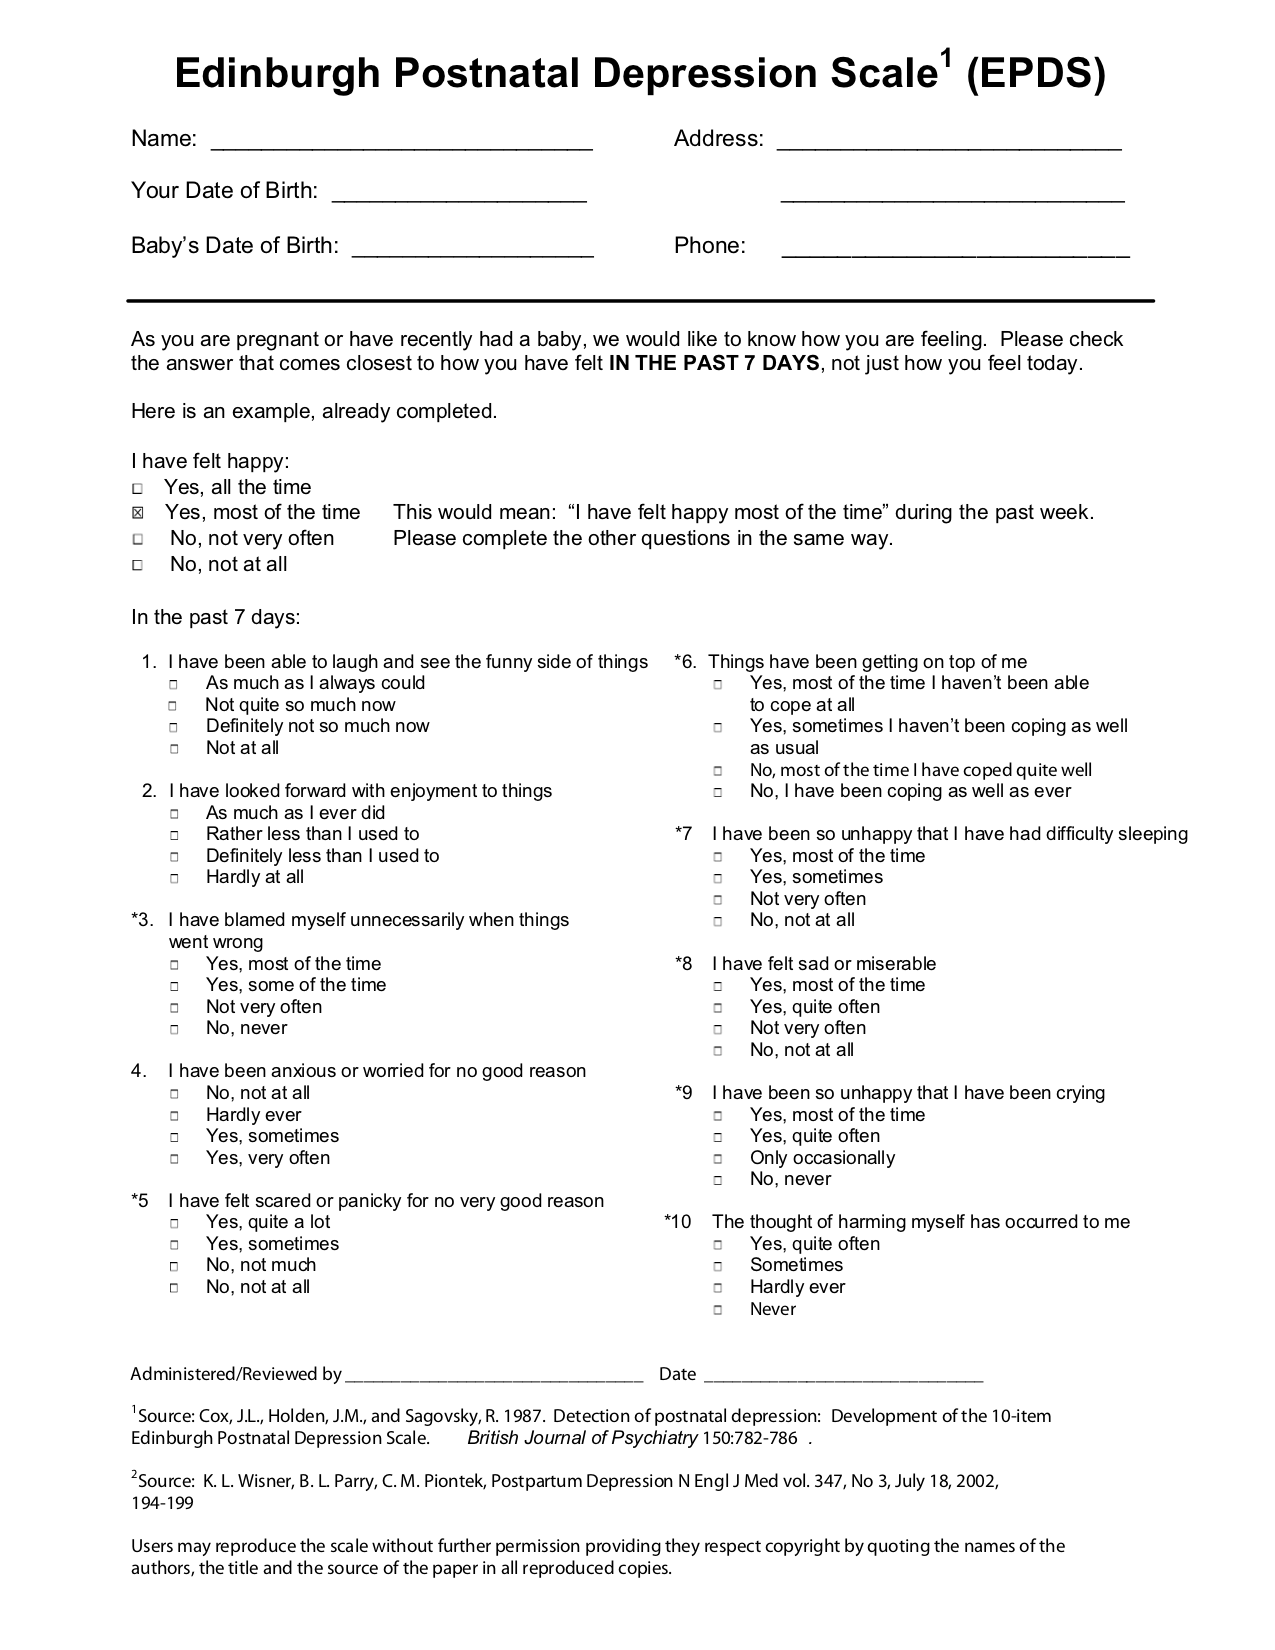
\includegraphics[width=13.8cm,height=16cm]{Figure1.png}
\end{center}

\begin{center}
	\hspace*{-2.1cm}
 	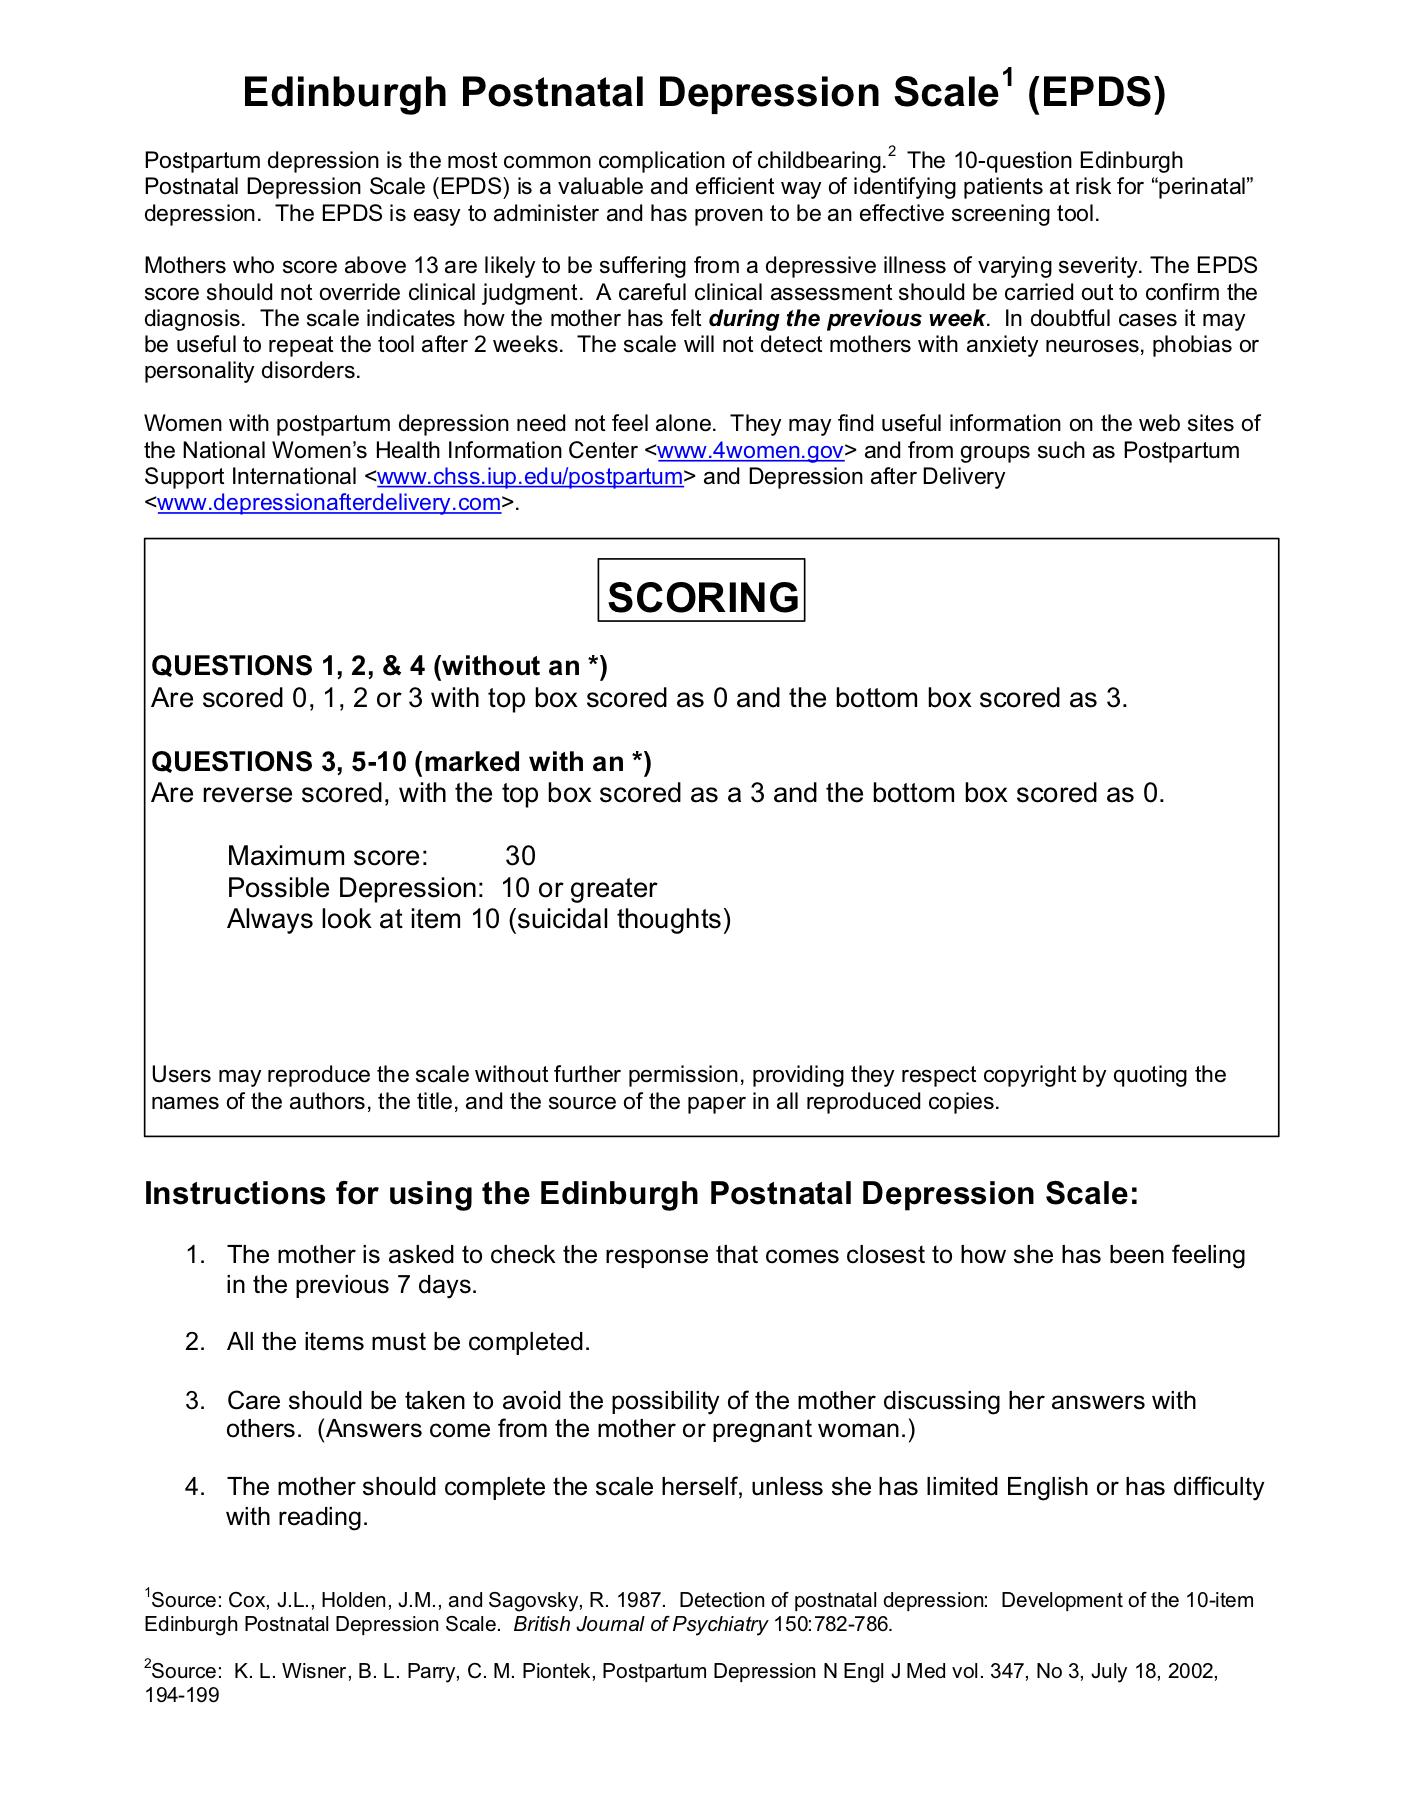
\includegraphics[width=18cm,height=21.2cm]{Figure2.png}
\end{center}

\chapter{Código R}
%[formatcom=\color{Blue}]
\begin{Verbatim}

#####################################################################
########## ANÁLISIS DE DATOS ESTUDIO DEPRESIÓN POSTPARTO ###########
#####################################################################

# -------- 0. PAQUETES NECESARIOS. -------- #
#install.packages("epiDisplay")
library(epiDisplay)
#install.packages("logbin")
library(logbin)


# -------- 1. LECTURA DE DATOS. -------- #
load("DPP.RData")
head(dppdat)
labels(dppdat)
summary(dppdat)


# -------- 2. MODELOS DE REGRESIÓN LOGÍSTICA. -------- #
### 2.1. Síntomas de depresión a las 8 semanas (EPDS>9).
logistica8 <- glm(epds8wc~epqnT+epds0+duke+antpers, data=dppdat,
family=binomial(link="logit"))
summary(logistica8)
logistic.display(logistica8)

### 2.2. Síntomas de depresión a las 32 semanas (EPDS>9).
logistica32 <- glm(epds32winc~epqnT+epds0+ecoprob, data=dppdat,
family=binomial(link="logit"))
summary(logistica32)
logistic.display(logistica32)

### 2.3. Diagnóstico clínico de la depresión postparto (DIGS).
logisticaDIGS <- glm(digs0a32~epqnT+epds0+antpers+antpsifa+expvit, 
data=dppdat,family=binomial(link="logit"))
summary(logisticaDIGS)
logistic.display(logisticaDIGS)


# -------- 3. MODELOS DE REGRESIÓN LOG-BINOMIAL CON FUNCIÓN GLM. -------- #
### 3.1. Síntomas de depresión a las 8 semanas (EPDS>9).
logbinonial8 <- glm(epds8wc~epqnT+epds0+duke+antpers, data=dppdat,
 family=binomial(link="log"))
summary(logbinonial8)
exp(coef(logbinonial8))[-1]

##### Con argumento "start".
logbinonial8.start1 <- glm(epds8wc~epqnT+epds0+duke+antpers, data=dppdat, 
family=binomial(link="log"), start=c(-4, rep(0,4)))
summary(logbinonial8.start1)
exp(coef(logbinonial8.start1))[-1]


### 3.2. Síntomas de depresión a las 32 semanas (EPDS>9).
logbinomial32 <- glm(epds32winc~epqnT+epds0+ecoprob, data=dppdat, 
family=binomial(link="log"))
summary(logbinomial32)
exp(coef(logbinomial32))[-1]


### 3.3. Diagnóstico clínico de la depresión postparto (DIGS).
logbinomialDIGS <- glm(digs0a32~epqnT+epds0+antpers+antpsifa+expvit,
 data=dppdat, family=binomial(link="log"))
summary(logbinomialDIGS)
exp(coef(logbinomialDIGS))[-1]

##### Con argumento start.
logbinomialDIGS.start1 <- glm(digs0a32~epqnT+epds0+antpers+antpsifa+expvit, 
data=dppdat, family=binomial(link="log"), start=c(-4, rep(0,5)))
summary(logbinomialDIGS.start1)
exp(coef(logbinomialDIGS.start1))[-1]


# -------- 4. MODELOS DE REGRESIÓN LOG-BINOMIAL CON FUNCIÓN LOGBIN. -------- #
### 4.1. Síntomas de depresión a las 8 semanas (EPDS>9).
logbin8 <- logbin(epds8wc~epqnT+epds0+duke+antpers, data=dppdat)
summary(logbin8)
exp(coef(logbin8))[-1]

##### Con argumento bound.tol.
logbin8.bound <- logbin(epds8wc~epqnT+epds0+duke+antpers, data=dppdat, 
bound.tol= 0.05)
summary(logbin8.bound)
exp(coef(logbin8.bound))[-1]

### 4.2. Síntomas de depresión a las 32 semanas (EPDS>9).
logbin32 <- logbin(epds32winc~epqnT+epds0+ecoprob, data=dppdat)
summary(logbin32)
exp(coef(logbin32))[-1]

### 4.3. Diagnóstico clínico de la depresión postparto (DIGS).
logbinDIGS <- logbin(digs0a32~epqnT+epds0+antpers+antpsifa+expvit, data=dppdat)
summary(logbinDIGS)
exp(coef(logbinDIGS))[-1]

##### Con argumentos "bound.tol" y "maxit".
logbinDIGS.bound <- logbin(digs0a32~epqnT+epds0+antpers+antpsifa+expvit, 
data=dppdat, maxit=100, bound.tol= 0.05)
summary(logbinDIGS.bound)
exp(coef(logbinDIGS.bound))[-1]


# -------- 5. MODELOS DE REGRESIÓN LOG-BINOMIAL CON FUNCIÓN COPY. -------- #
### 5.1. Creación de la función COPY.
copy <- function(data, Y, vars,n, W) {
	if (!is.numeric(data[, Y])) {
		data[, Y] <- as.numeric(data[, Y])-1
	}
	data$W <- (n-1)/n
	data.copy <- data
	data.copy[, Y] <- 1-data.copy[, Y]
	data.copy$W <- 1/n
	data.all <- merge(data, data.copy, all = T)
	formul <- paste(Y, paste(vars, collapse = " + "), sep = "~")
	mod.mat <- model.matrix(as.formula(formul), data)
	glm.copy <- glm(as.formula(formul), family = binomial(log), data.all,
		    weights = W, control = list(maxit = 100),
		    start = c(-4, rep(0, ncol(mod.mat)-1)))
	return(glm.copy)
}

### 5.2. Síntomas de depresión a las 8 semanas (EPDS>9).
##### 5.2.1.Con n=100 copias.
logbinonial8.copy100 <- copy(dppdat,'epds8wc', vars = c('epqnT','epds0',
'duke','antpers'),100)
summary(logbinonial8.copy100)
exp(coef(logbinonial8.copy100))[-1]

##### 5.2.2.Con n=1000 copias.
logbinonial8.copy1000 <- copy(dppdat,'epds8wc', vars = c('epqnT','epds0',
'duke','antpers'),1000)
summary(logbinonial8.copy1000)
exp(coef(logbinonial8.copy1000))[-1]

##### 5.2.3.Con n=10000 copias.
logbinonial8.copy10000 <- copy(dppdat,'epds8wc', vars = c('epqnT','epds0',
'duke','antpers'),10000)
summary(logbinonial8.copy10000)
exp(coef(logbinonial8.copy10000))[-1]


### 5.3. Síntomas de depresión a las 32 semanas (EPDS>9).
##### 5.3.1.Con n=100 copias.
logbinonial32.copy100 <- copy(dppdat,'epds32winc', vars = c('epqnT','epds0',
'ecoprob'),100)
summary(logbinonial32.copy100)
exp(coef(logbinonial32.copy100))[-1]

##### 5.3.2.Con n=1000 copias.
logbinonial32.copy1000 <- copy(dppdat,'epds32winc', vars = c('epqnT','epds0',
'ecoprob'),1000)
summary(logbinonial32.copy1000)
exp(coef(logbinonial32.copy1000))[-1]

###### 5.3.3.Con n=10000 copias.
logbinonial32.copy10000 <- copy(dppdat,'epds32winc', vars = c('epqnT','epds0',
'ecoprob'),10000)
summary(logbinonial32.copy10000)
exp(coef(logbinonial32.copy10000))[-1]


### 5.4. Diagnóstico clínico de la depresión postparto (DIGS).
##### 5.4.1.Con n=100 copias.
logbinonialDIGS.copy100 <- copy(dppdat,'digs0a32', vars = c('epqnT','epds0',
'antpers','antpsifa','expvit'),100)
summary(logbinonialDIGS.copy100)
exp(coef(logbinonialDIGS.copy100))[-1]

##### 5.4.2.Con n=1000 copias.
logbinonialDIGS.copy1000 <- copy(dppdat,'digs0a32', vars = c('epqnT','epds0',
'antpers','antpsifa','expvit'),1000)
summary(logbinonialDIGS.copy1000)
exp(coef(logbinonialDIGS.copy1000))[-1]

###### 5.4.3.Con n=10000 copias.
logbinonialDIGS.copy10000 <- copy(dppdat,'digs0a32', vars = c('epqnT','epds0',
'antpers','antpsifa','expvit'),10000)
summary(logbinonialDIGS.copy10000)
exp(coef(logbinonialDIGS.copy10000))[-1]


# -------- 6. PRESENCIA DE SEPARACIÓN EN LOS MODELOS LOG-BINOMIALES 1 Y 3. -------- #
#install.packages("safeBinaryRegression")
library(safeBinaryRegression)

### 6.1. Síntomas de depresión a las 8 semanas (EPDS>9).
glm(epds8wc~epqnT+epds0+duke+antpers, data=dppdat, family=binomial(link="log"), 
separation ="find")

### 6.2. Diagnóstico clínico de la depresión postparto (DIGS).
glm(digs0a32~epqnT+epds0+antpers+antpsifa+expvit, data=dppdat, family=
binomial(link="log"), separation ="find")

# -------- 7. PRUEBAS DE BONDAD DE AJUSTE CON HOSMER-LEMESHOW. -------- #
### 7.1. Modelos de regresión logística. 
hoslem.test(logistica8$y, fitted(logistica8), g=10)
hoslem.test(logistica32$y, fitted(logistica32), g=10)
hoslem.test(logisticaDIGS$y, fitted(logisticaDIGS), g=10)

### 7.2. Modelos de regresión log-binomial.
###### 7.2.1.Con función "glm".
hoslem.test(logbinonial8.start1$y, fitted(logbinonial8.start1), g=10)
hoslem.test(logbinomial32$y, fitted(logbinomial32), g=10)
hoslem.test(logbinomialDIGS.start1$y, fitted(logbinomialDIGS.start1), g=10)

###### 7.2.1.Con función "logbin".
hoslem.test(logbin8$y, fitted(logbin8), g=10) 
hoslem.test(logbin32$y, fitted(logbin32), g=10)
hoslem.test(logbinDIGS$y, fitted(logbinDIGS), g=10)

###### 7.2.1.Con función "COPY".
hoslem.test(logbinonial8.copy100$y, fitted(logbinonial8.copy100), g=10)
hoslem.test(logbinonial8.copy1000$y, fitted(logbinonial8.copy1000), g=10)
hoslem.test(logbinonial8.copy10000$y, fitted(logbinonial8.copy10000), g=10)

hoslem.test(logbinonial32.copy100$y, fitted(logbinonial32.copy100), g=10)
hoslem.test(logbinonial32.copy1000$y, fitted(logbinonial32.copy1000), g=10)
hoslem.test(logbinonial32.copy10000$y, fitted(logbinonial32.copy10000), g=10)

hoslem.test(logbinonialDIGS.copy100$y, fitted(logbinonialDIGS.copy100), g=10)
hoslem.test(logbinonialDIGS.copy1000$y, fitted(logbinonialDIGS.copy1000), g=10)
hoslem.test(logbinonialDIGS.copy10000$y, fitted(logbinonialDIGS.copy10000), g=10)
\end{Verbatim}

%--------------------------------------------------------------------------------
% PÁGINA EN BLANCO, FINAL DEL DOCUMENTO
%--------------------------------------------------------------------------------
\newpage
\thispagestyle{empty}
\mbox{}

\end{document}



